\documentclass{article}
\usepackage[utf8]{inputenc}
\usepackage{graphicx}
\usepackage{geometry}
\usepackage{amsmath}
\usepackage{amsfonts}
\usepackage{float}
\usepackage{caption}
\usepackage{subcaption}
\usepackage{enumitem}

\geometry{left=25mm, top=25mm, right=25mm, bottom=25mm}

\title{PHY407 Lab 9}
\author{Pierino Zindel (1002429703) and Hayden Johnson (1002103537)}
\date{November 16, 2018}

\begin{document}

\maketitle

\noindent \textbf{Distribution of work:} Questions 1 and 3 were completed by Pierino. Question 2 was completed by Hayden.

\section{Solving the wave equation with the spectral method}
We desire to solve the wave equation 
\begin{equation}
	\label{eq:wave}
	\frac{\partial^2 \phi}{\partial t^2} = v^2 \frac{\partial^2 \phi}{\partial x^2}
\end{equation}
similar to Q2 of Lab08, using the spectral method. The initial conditions of our problem are 
\begin{equation}
\label{eq:phi_0}
	\phi (x,t=0) = \phi _0(x)= \sum^{\infty} _{k=1} \widetilde{ \phi } _{0,k} \sin ( \frac{k \pi x}{L})
\end{equation}
and 
\begin{equation}
\label{eq:psi_0}
	\frac{\partial \phi(x,t=0)}{\partial t} = \psi_0(x) = \sum^{\infty}_{k=1} \widetilde{\psi}_{0,k} \sin(\frac{k\pi x}{L})
\end{equation}
satisfying the boundary condition
\begin{equation}
	\phi(x=0,t)=0=\phi(x=L,t)
\end{equation}

\subsection{Part a)}
We can confirm that the general solution to our problem in terms of the Fourier series is 
\begin{equation}
	\label{eq:general_solution}
	\phi(x,t)= \sum^{\infty}_{k=1} \sin(\frac{k\pi x}{L}) \left[ \widetilde{\phi}_{0,k} \cos(\omega_k t) + \frac{\widetilde{\psi}_{0,k}}{\omega_k} \sin(\omega_k t) \right]
\end{equation}

by showing that it satisfies the initial and boundary conditions.

First looking at the boundary conditions we see that when $x=0$ and $x=L$ the term $\sin(k\pi)$ in equation \ref{eq:general_solution} is zero and thus the boundary condition is satisfied.

Next we confirm the initial condition by letting $t=0$ in equation \ref{eq:general_solution} to get 
\begin{equation}
\begin{split}
	\phi(x,t=0)=& \sum^{\infty}_{k=1} \sin(\frac{k\pi x}{L}) \left[\widetilde{\phi}_{0,k} + 0 \right]
	\\ =& \phi_0(x)
\end{split}
\end{equation}

Then taking the partial derivative with respect to time we have

\begin{equation}
\begin{split}
	\psi(x,t=0) =& \frac{\partial \phi(x,t=0)}{\partial t}
	\\ =& \sum^{\infty}_{k=1} \sin(\frac{k\pi x}{L}) \left[-\omega_k \widetilde{\phi}_{0,k} \sin(\omega_k t) + \widetilde{\psi}_{0,k} \cos(\omega_k t) \right]
	\\ =& \sum^{\infty}_{k=1} \sin(\frac{k\pi x}{L}) \left[0 + \widetilde{\psi}_{0,k} \right]
	\\ =& \psi_0(x)
\end{split}
\end{equation}

and thus the initial conditions are also satisfied by the general solution equation \ref{eq:general_solution}.

Having shown that the solution given is valid we now apply the wave equation to it and derive an expression for the frequency $\omega_k$ in terms of $k$, $L$, and $v$.

Starting with the time derivative component we get
\begin{equation}
\begin{split}
	\frac{\partial^2 \phi}{\partial t^2} =& \sum^{\infty}_{k=1} \sin(\frac{k\pi x}{L}) \left[-\omega_k^2 \widetilde{\phi}_{0,k} \cos(\omega_k t) - \omega_k \widetilde{\psi}_{0,k} \sin(\omega_k t) \right]
	\\ =& - \omega_k^2 \phi(x,t)
\end{split}
\end{equation}

and the $x$ derivative component gives us

\begin{equation}
\begin{split}
	\frac{ \partial^2 \phi }{ \partial x^2} =& \sum^{\infty}_{k=1} \left( \frac{k\pi}{L} \right)^2 \sin(\frac{k\pi x}{L}) \left[ \widetilde{\phi}_{0,k} \cos(\omega_k t) + \frac{\widetilde{\psi}_{0,k}}{\omega_k} \sin(\omega_k t) \right]
	\\ =& - \left( \frac{k \pi}{L} \right)^2 \phi(x,t)
\end{split}
\end{equation}

We then combine these into the wave equation to get

\begin{equation}
\begin{split}
	\frac{\partial^2 \phi}{\partial t^2} =& v^2 \frac{\partial^2 \phi}{\partial x^2}
	\\ -\omega_k^2 \phi(x,t) =& - v^2 \left( \frac{k \pi}{L} \right)^2 \phi(x,t)
	\\ \omega_k =& \frac{k \pi v}{L}
\end{split}
\end{equation}

as our relation for $\omega_k$.

\subsection{Part b)}
Using the same problem as question 2 in Lab08 we have the parameters $v=100$m/s, $L=1$m, $N=100$, with initial conditions $\phi_0(x) = 0$ and 

\begin{equation}
	\psi_0(x) = C\frac{x(L-x)}{L^2}exp(-\frac{(x-d)^2}{2\sigma^2})
\end{equation}

where $d=0.1$m, $C=1.0$m/s, $\sigma=0.3$m.

The discrete sine transform from the provided dcst.py module is then applied to equations \ref{eq:phi_0} and \ref{eq:psi_0} with the initial conditions to retrieve the corresponding coefficients $\widetilde{\phi}_{0,k}$ and $\widetilde{\psi}_{0,k}$. These coefficients are then used in conjunction with the values for $\omega_k$ to find the coefficients

\begin{equation}
	c_k = \left[ \widetilde{\phi}_{0,k} \cos(\omega_k t) + \frac{\widetilde{\psi}_{0,k}}{\omega_k} \sin(\omega_k t) \right]
\end{equation}

for $k=0,..,N$. The inverse discrete sine transform is then used with the coefficients $c_k$ to get our solution $\phi$ for the wave equation.

The solutions for the times $t=2,4,6,12,100$ms  are shown in figure \ref{fig:wave_FT}. The solution for the same times that were computed using the FTCS method from Lab08 are shown in figure \ref{fig:wave_FTCS}. Comparing the two methods we can see that the FTCS grows increasingly unstable and at the time $t=100$ms the solution is overshadowed by the noise of the FTCS method, whereas the spectral method remains stable over the whole time interval.

The difference between the two methods, FTCS and spectral, is that the FTCS is a finite difference method that solves a pde by stepping through time with each subsequent step depending on the previous step. The spectral method has the benefit of not being a finite difference method allowing us to solve the equation for any desired time without having to solve the previous steps.

However, though the spectral method allows us to solve for a subset of times each step in the spectral method has a running time of $N\log N$ which means if we use $N$ sufficiently large and wish to solve for every step from $t=0$ to $t=T_{final}$ then the FTCS method would be faster given that each of its step only has a running time of $N$.

Another major disadvantage of the spectral method is that the problems it can be used to solve are limited to those that are linear with simple boundary conditions since the solution requires adding several individual solutions to get the final solution. The FTCS method doesn't depend on a linear combination of individual solutions and thus can be used to solve both linear and non-linear problems.

\begin{figure}[H] 	 
	\begin{minipage}[b]{0.33\linewidth}
  		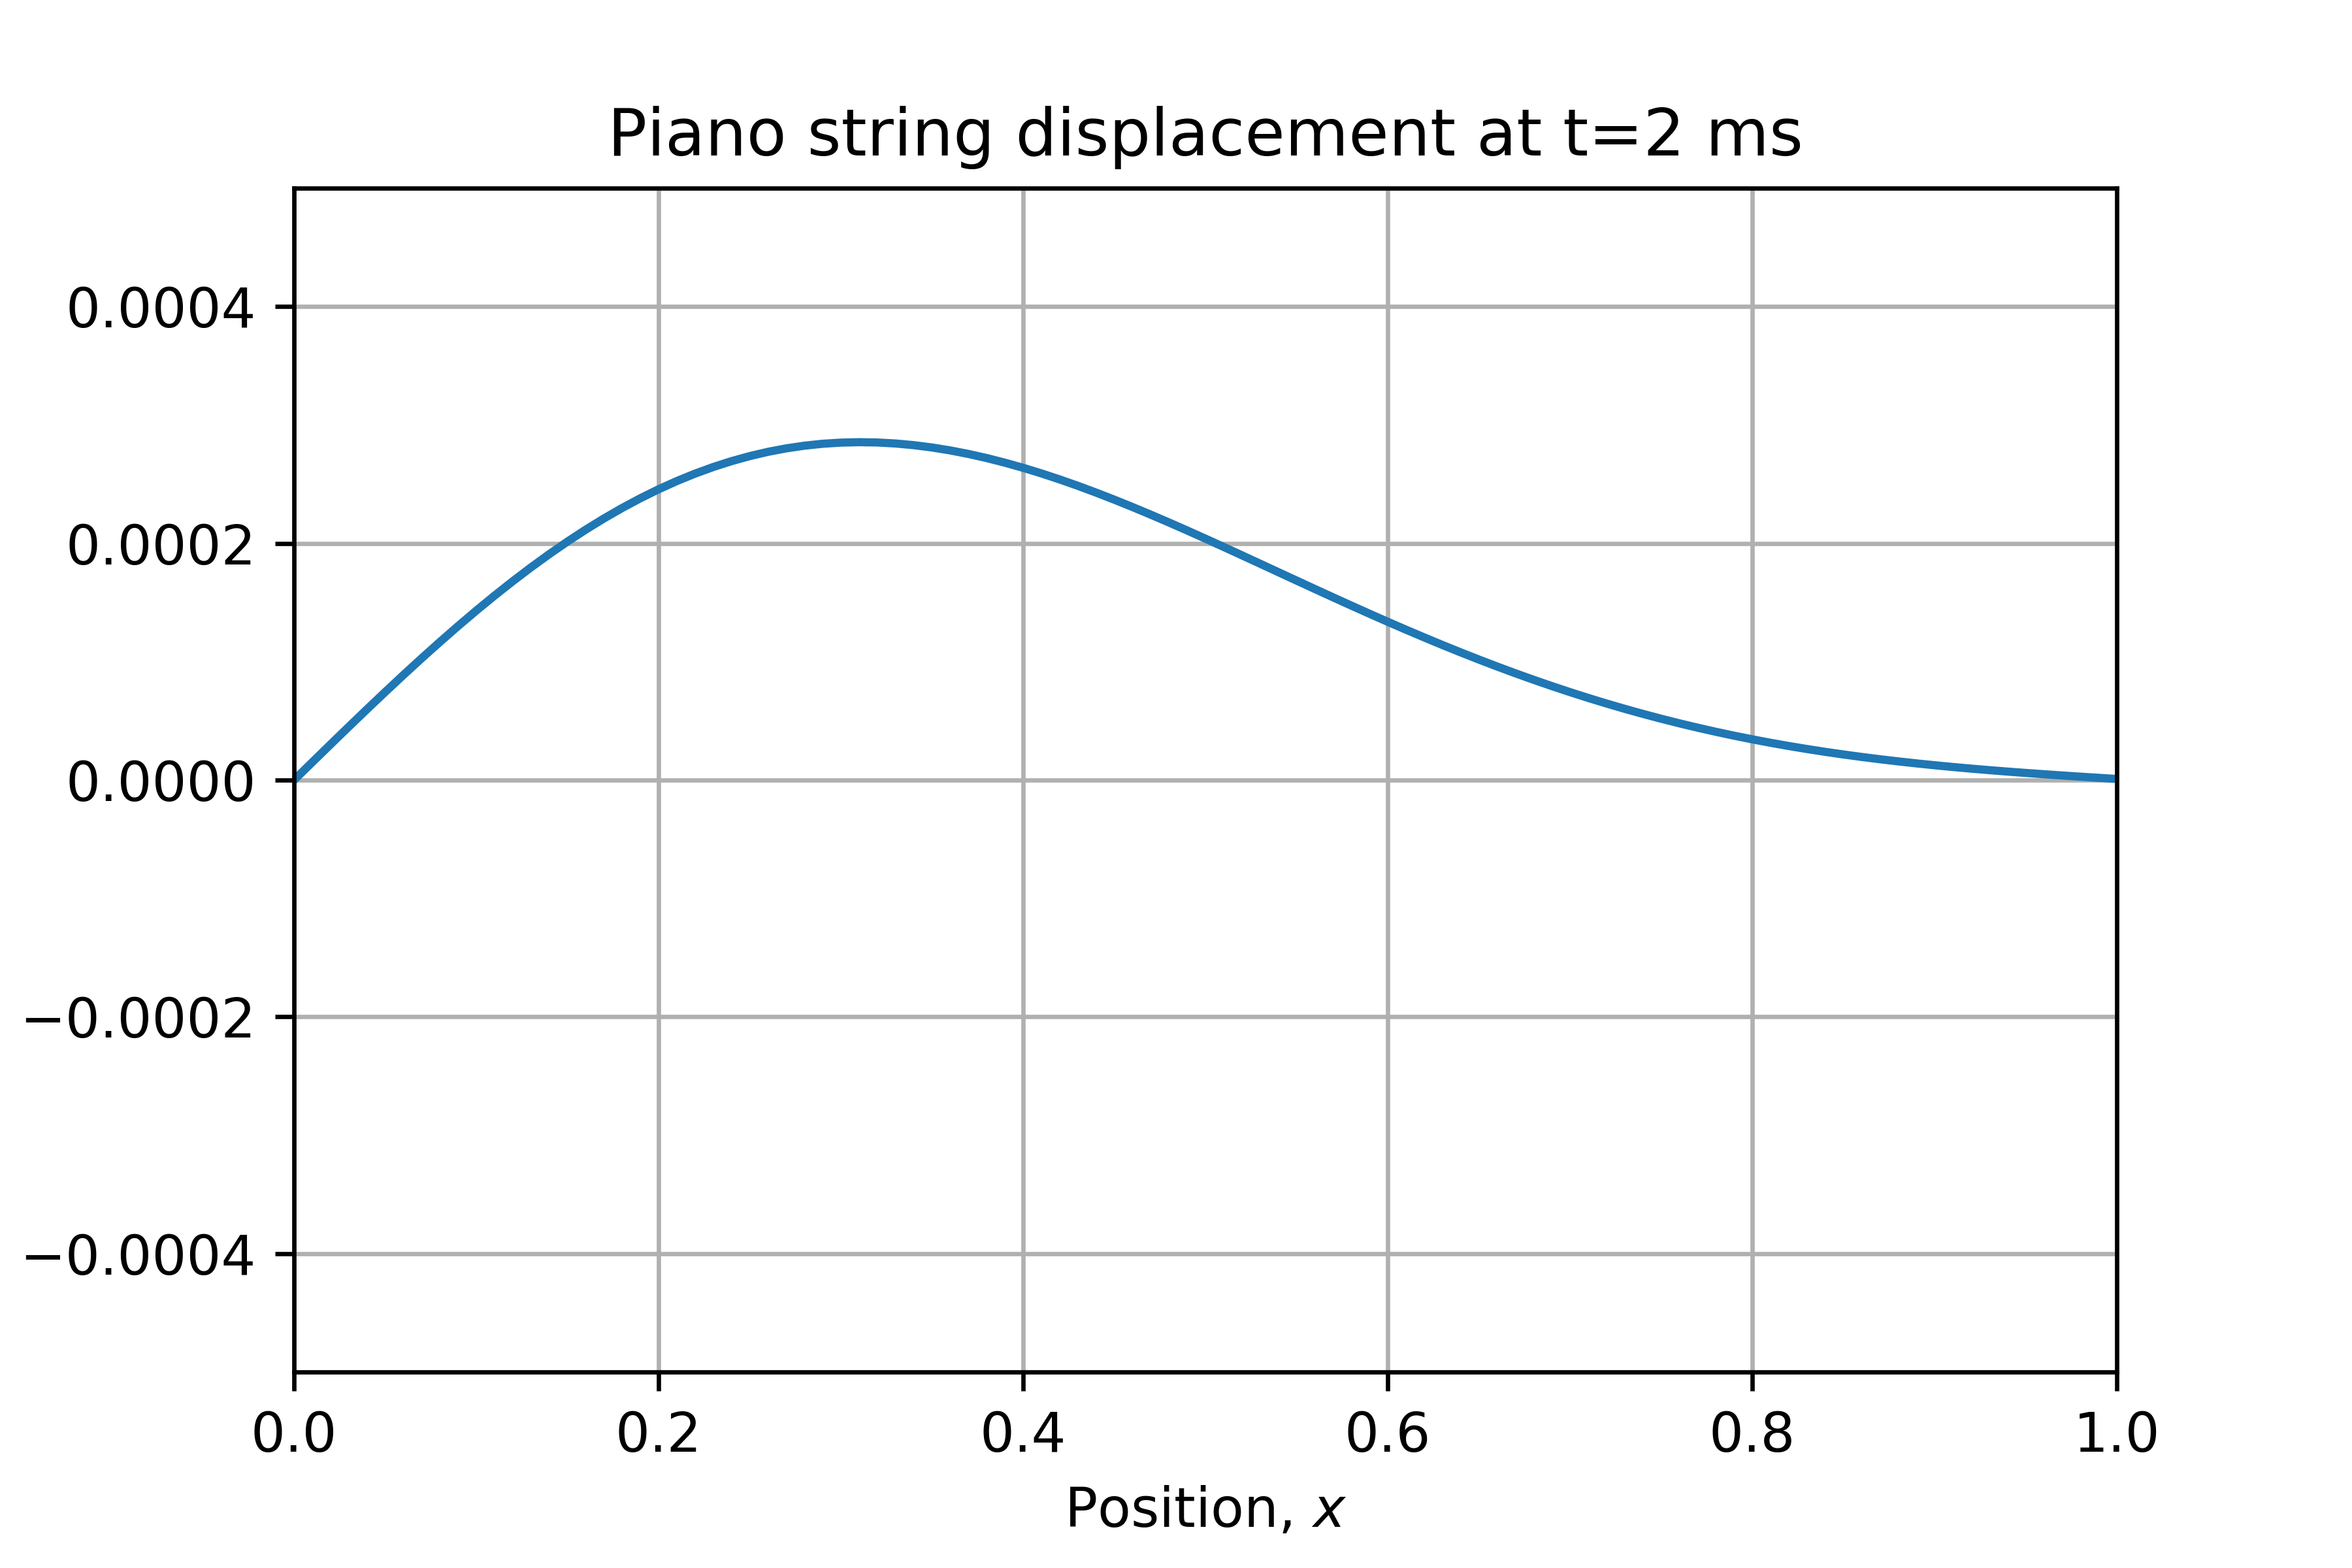
\includegraphics[width=1.0\linewidth]{../images/wave_eqtn_2ms.png} 
  	\end{minipage} 
  	\begin{minipage}[b]{0.33\linewidth}
    	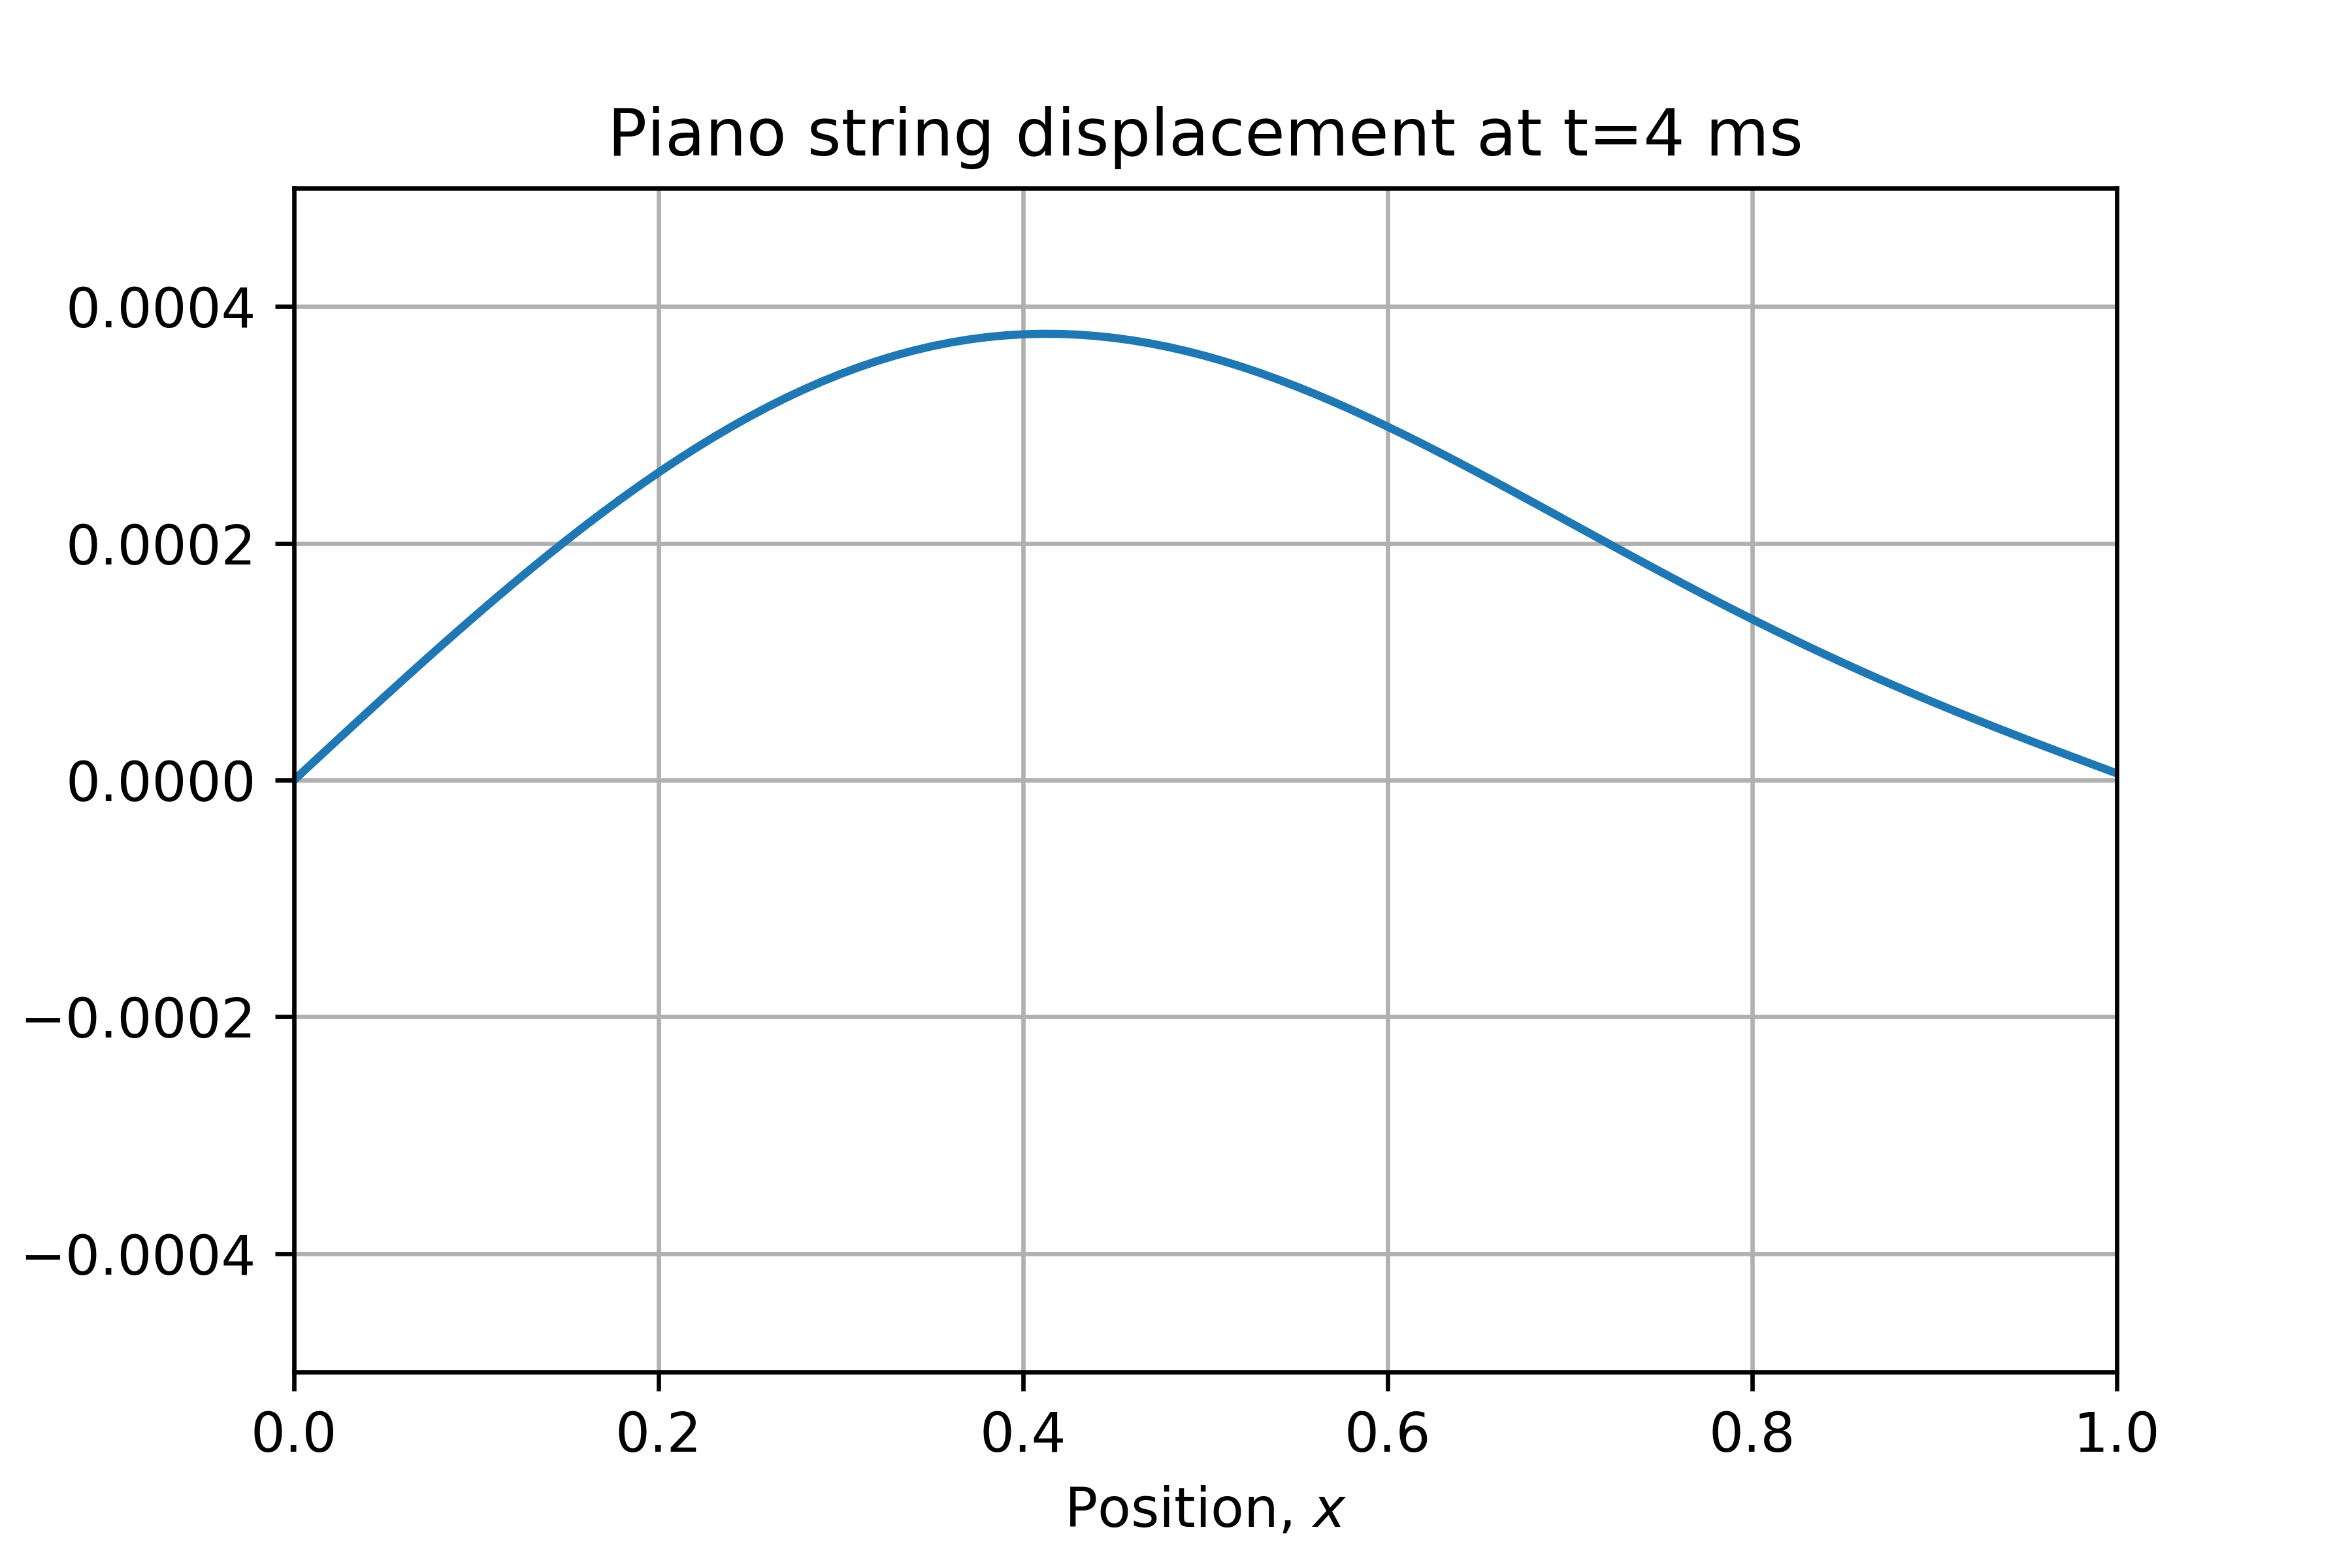
\includegraphics[width=1.0\linewidth]{../images/wave_eqtn_4ms.png} 
  	\end{minipage} 
  	\begin{minipage}[b]{0.33\linewidth}
    	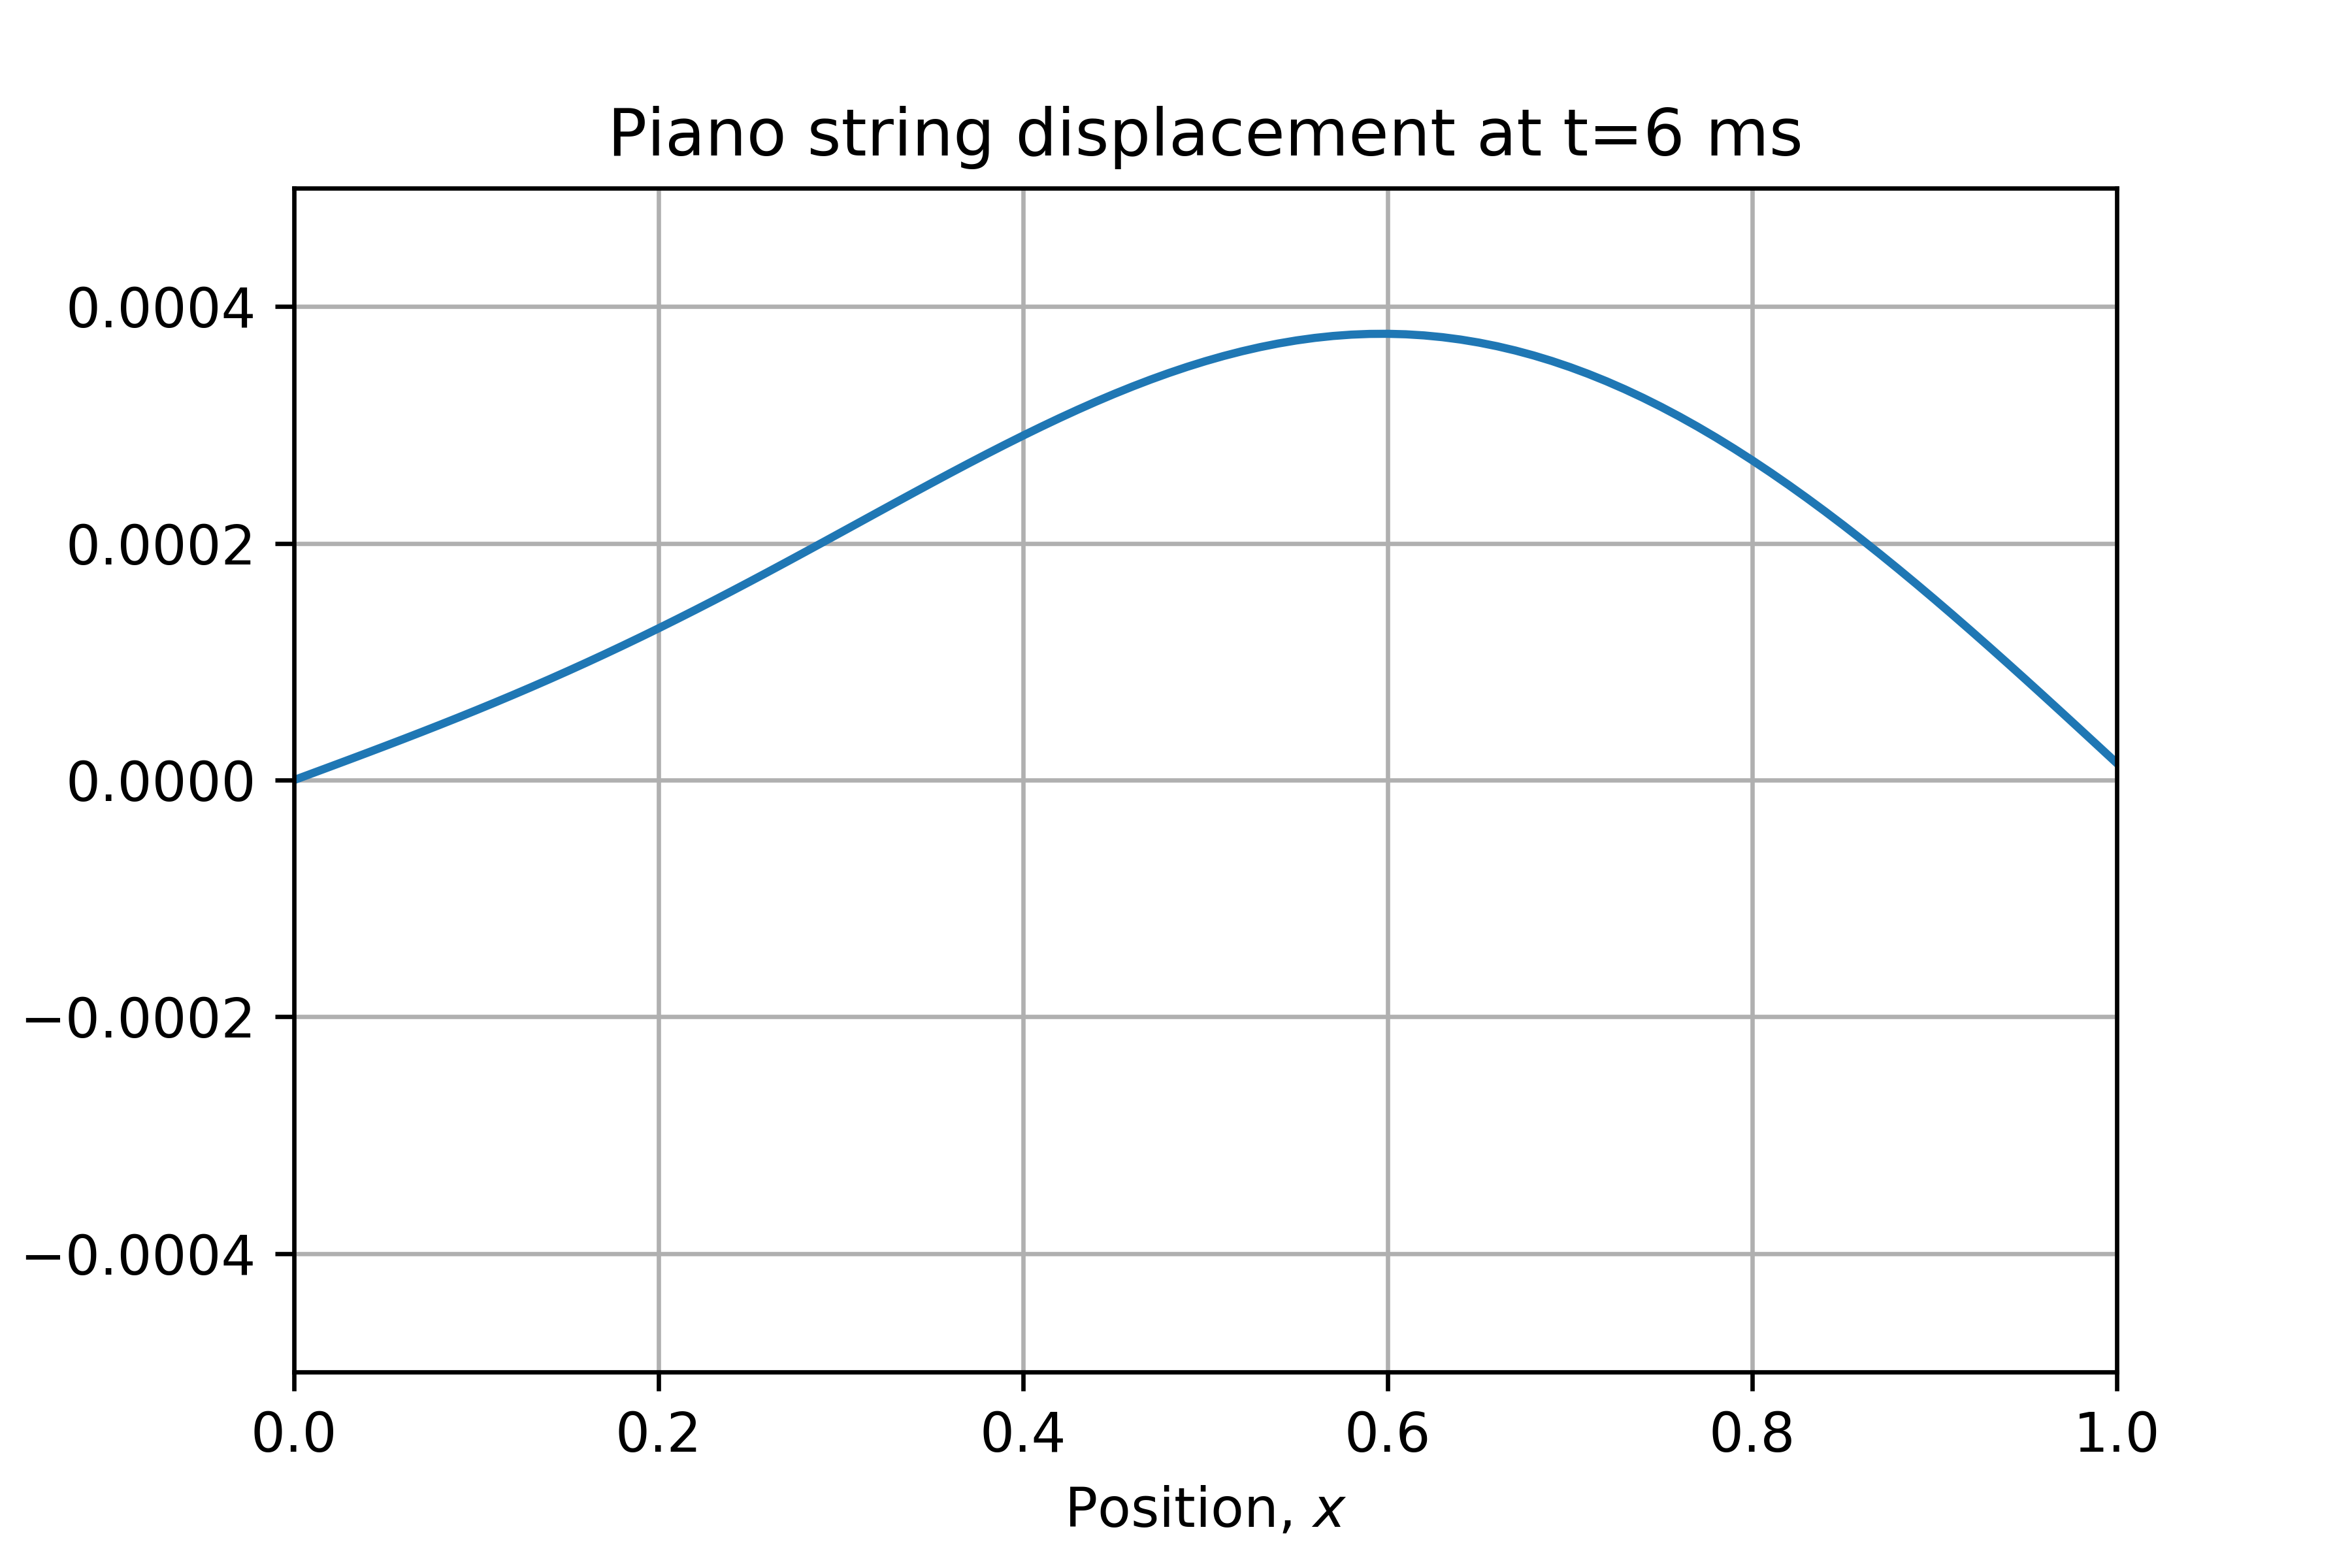
\includegraphics[width=1.0\linewidth]{../images/wave_eqtn_6ms.png}
  	\end{minipage}
  	\begin{minipage}[b]{0.33\linewidth}
    	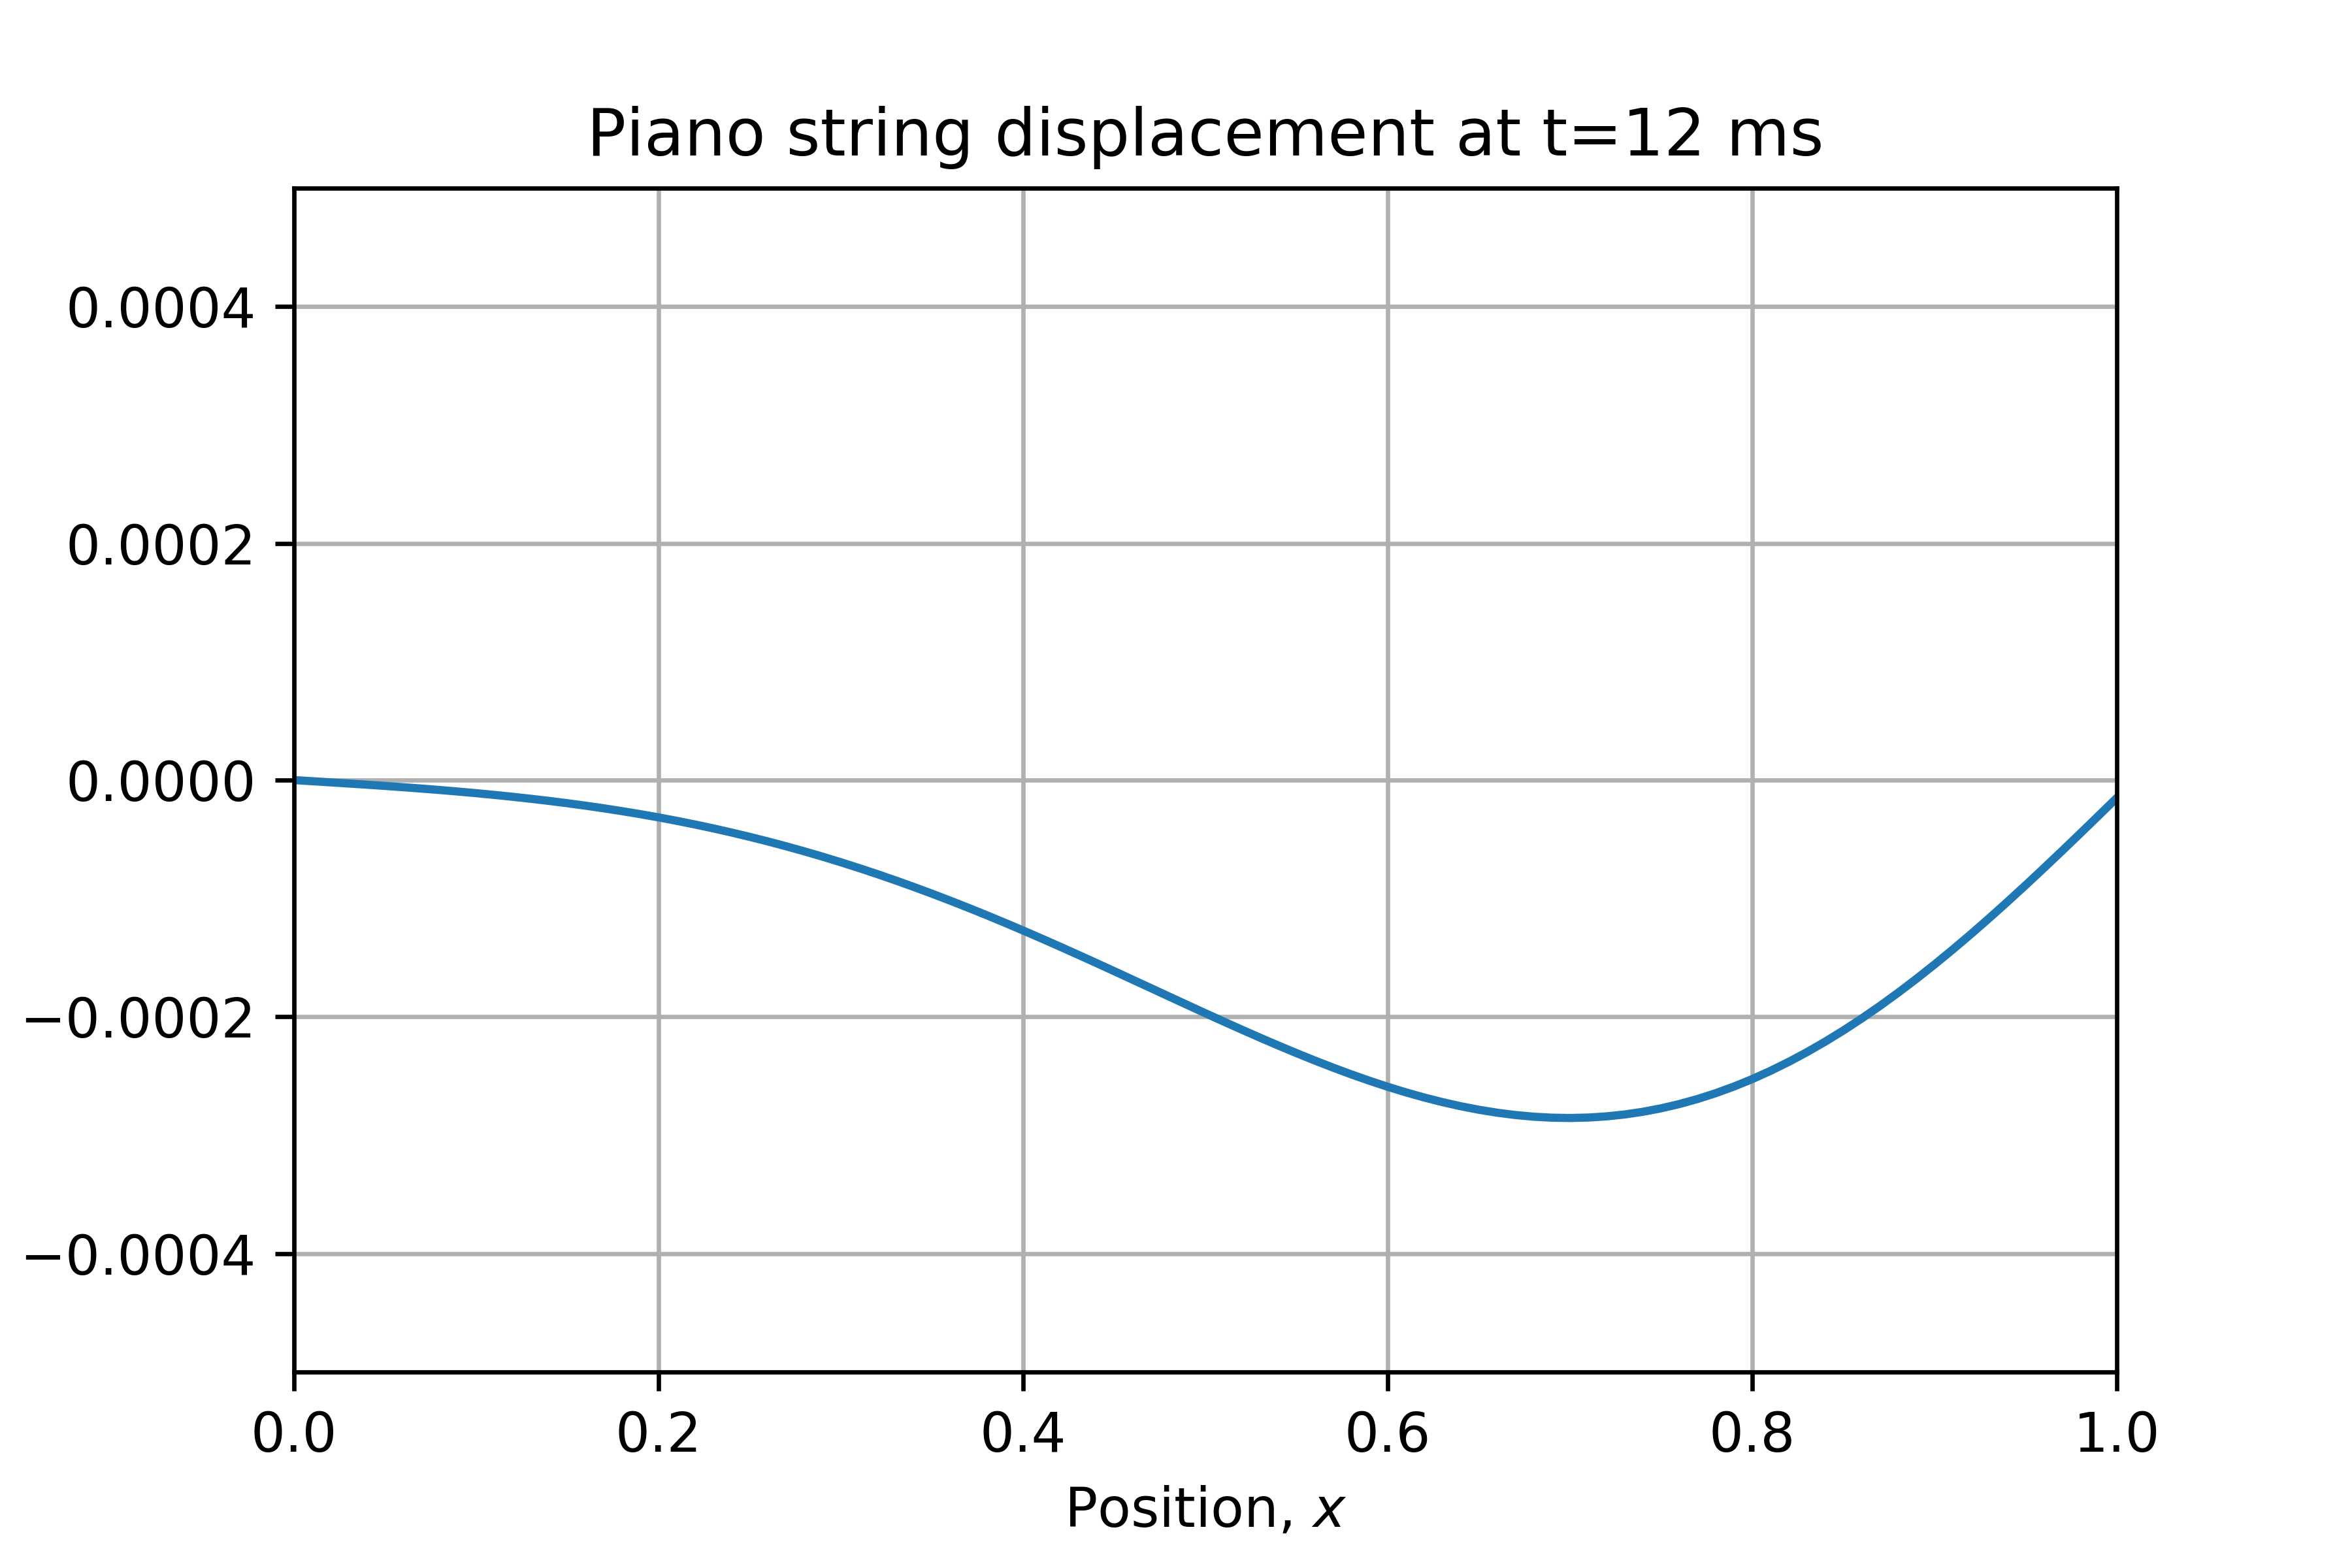
\includegraphics[width=1.0\linewidth]{../images/wave_eqtn_12ms.png} 
  	\end{minipage}
  	\begin{minipage}[b]{0.33\linewidth}
  		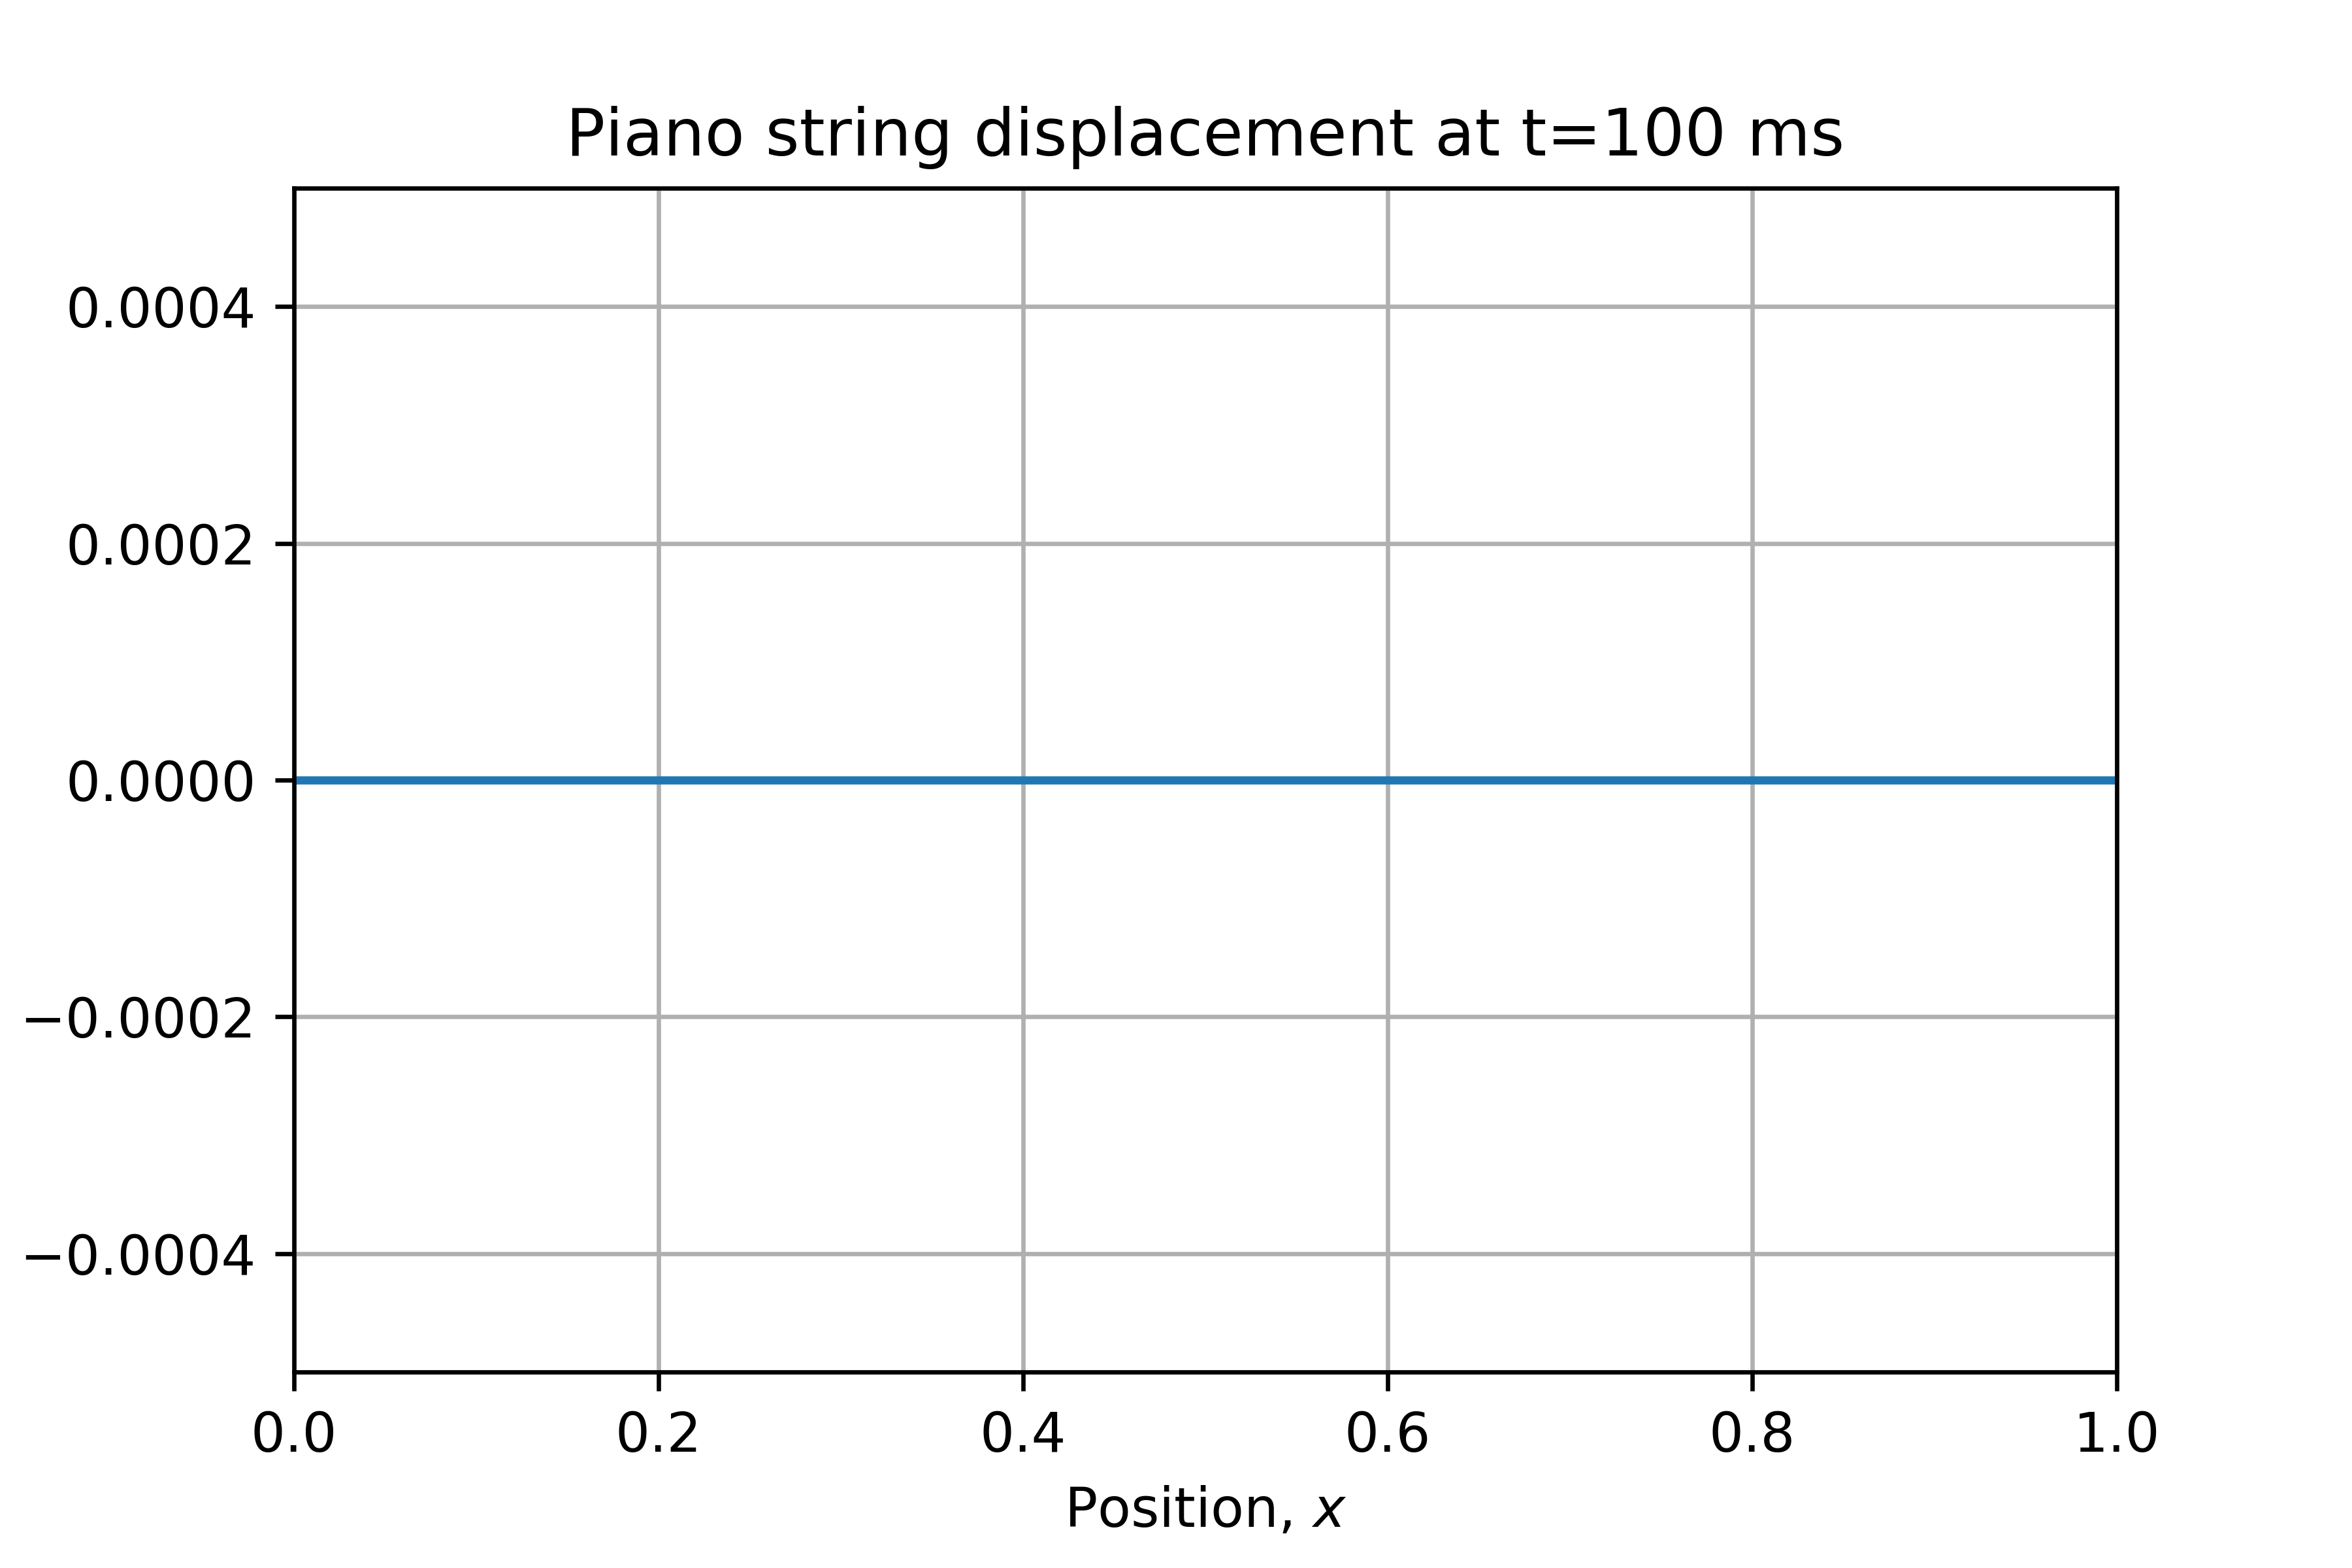
\includegraphics[width=1.0\linewidth]{../images/wave_eqtn_100ms.png}
  	\end{minipage}
 	\caption{Solution of the wave equation applied to the displacement of a struck piano string solved using the spectral method. Plotted for the times t = 2, 4, 6, 12, 100 milliseconds.} 
\label{fig:wave_FT}
\end{figure}


\begin{figure}[H]  
	\begin{minipage}[b]{0.33\linewidth}
  		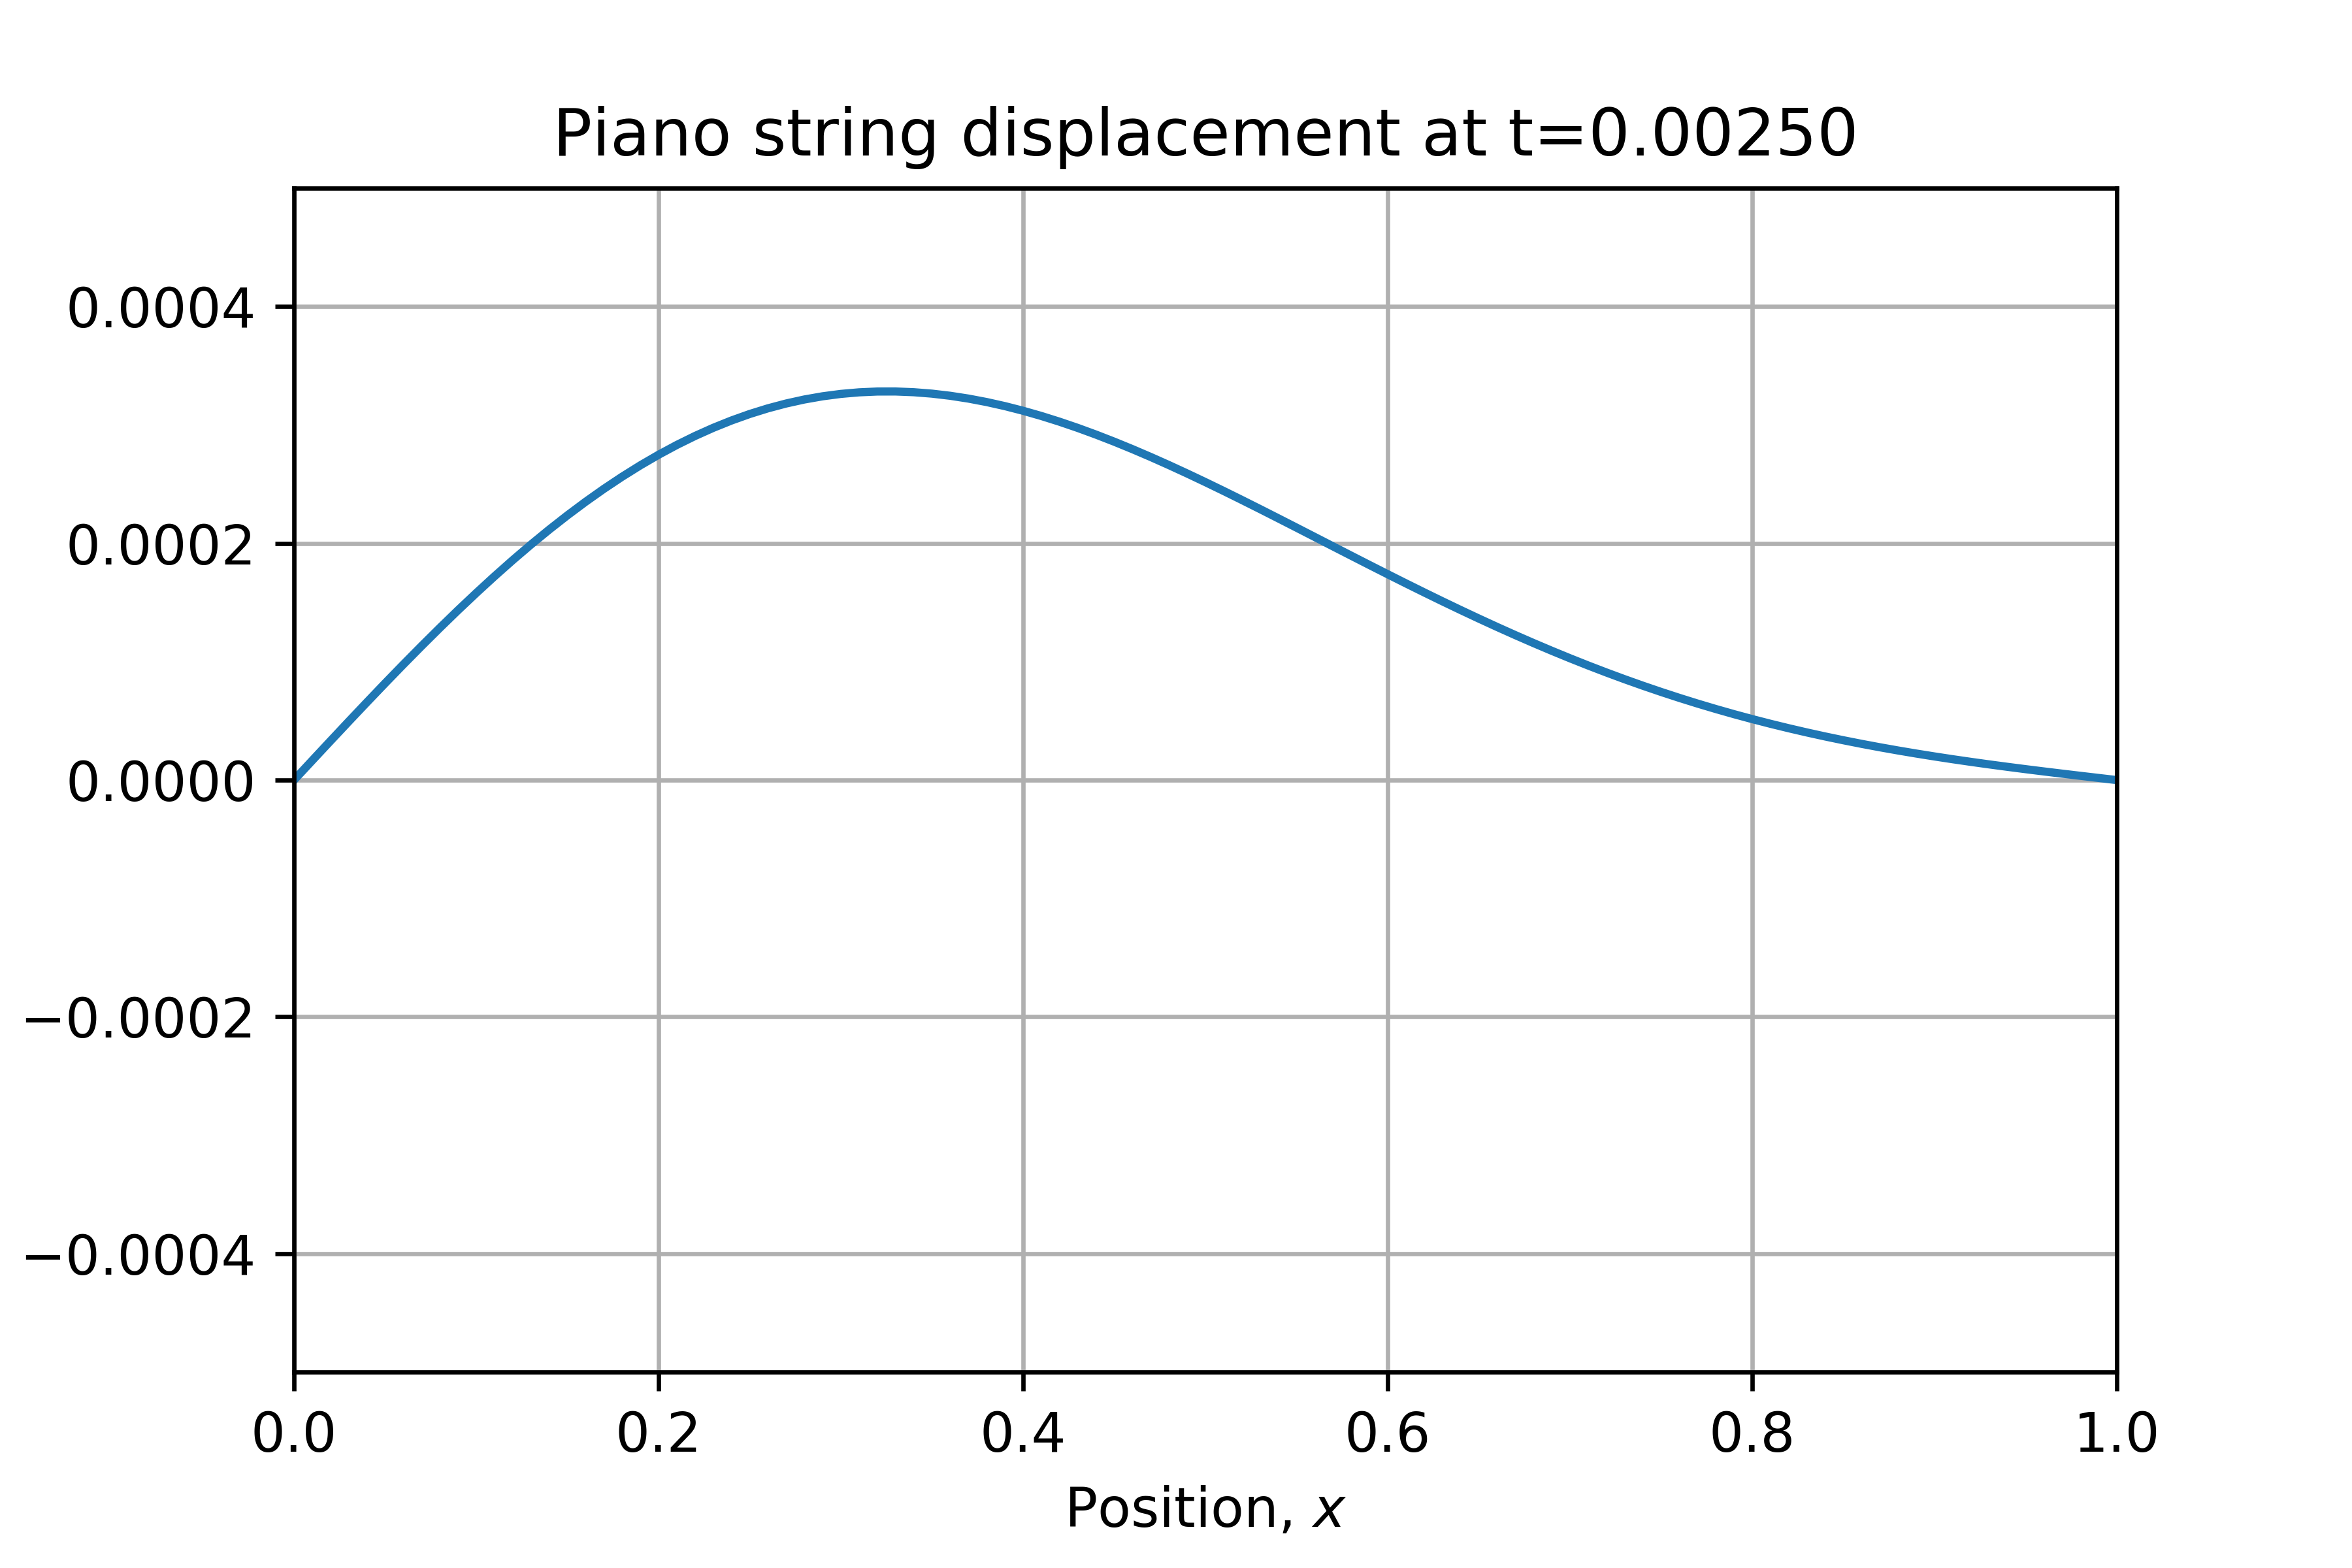
\includegraphics[width=1.0\linewidth]{../images/Lab08_t=2ms.png} 
  	\end{minipage} 
  	\begin{minipage}[b]{0.33\linewidth}
    	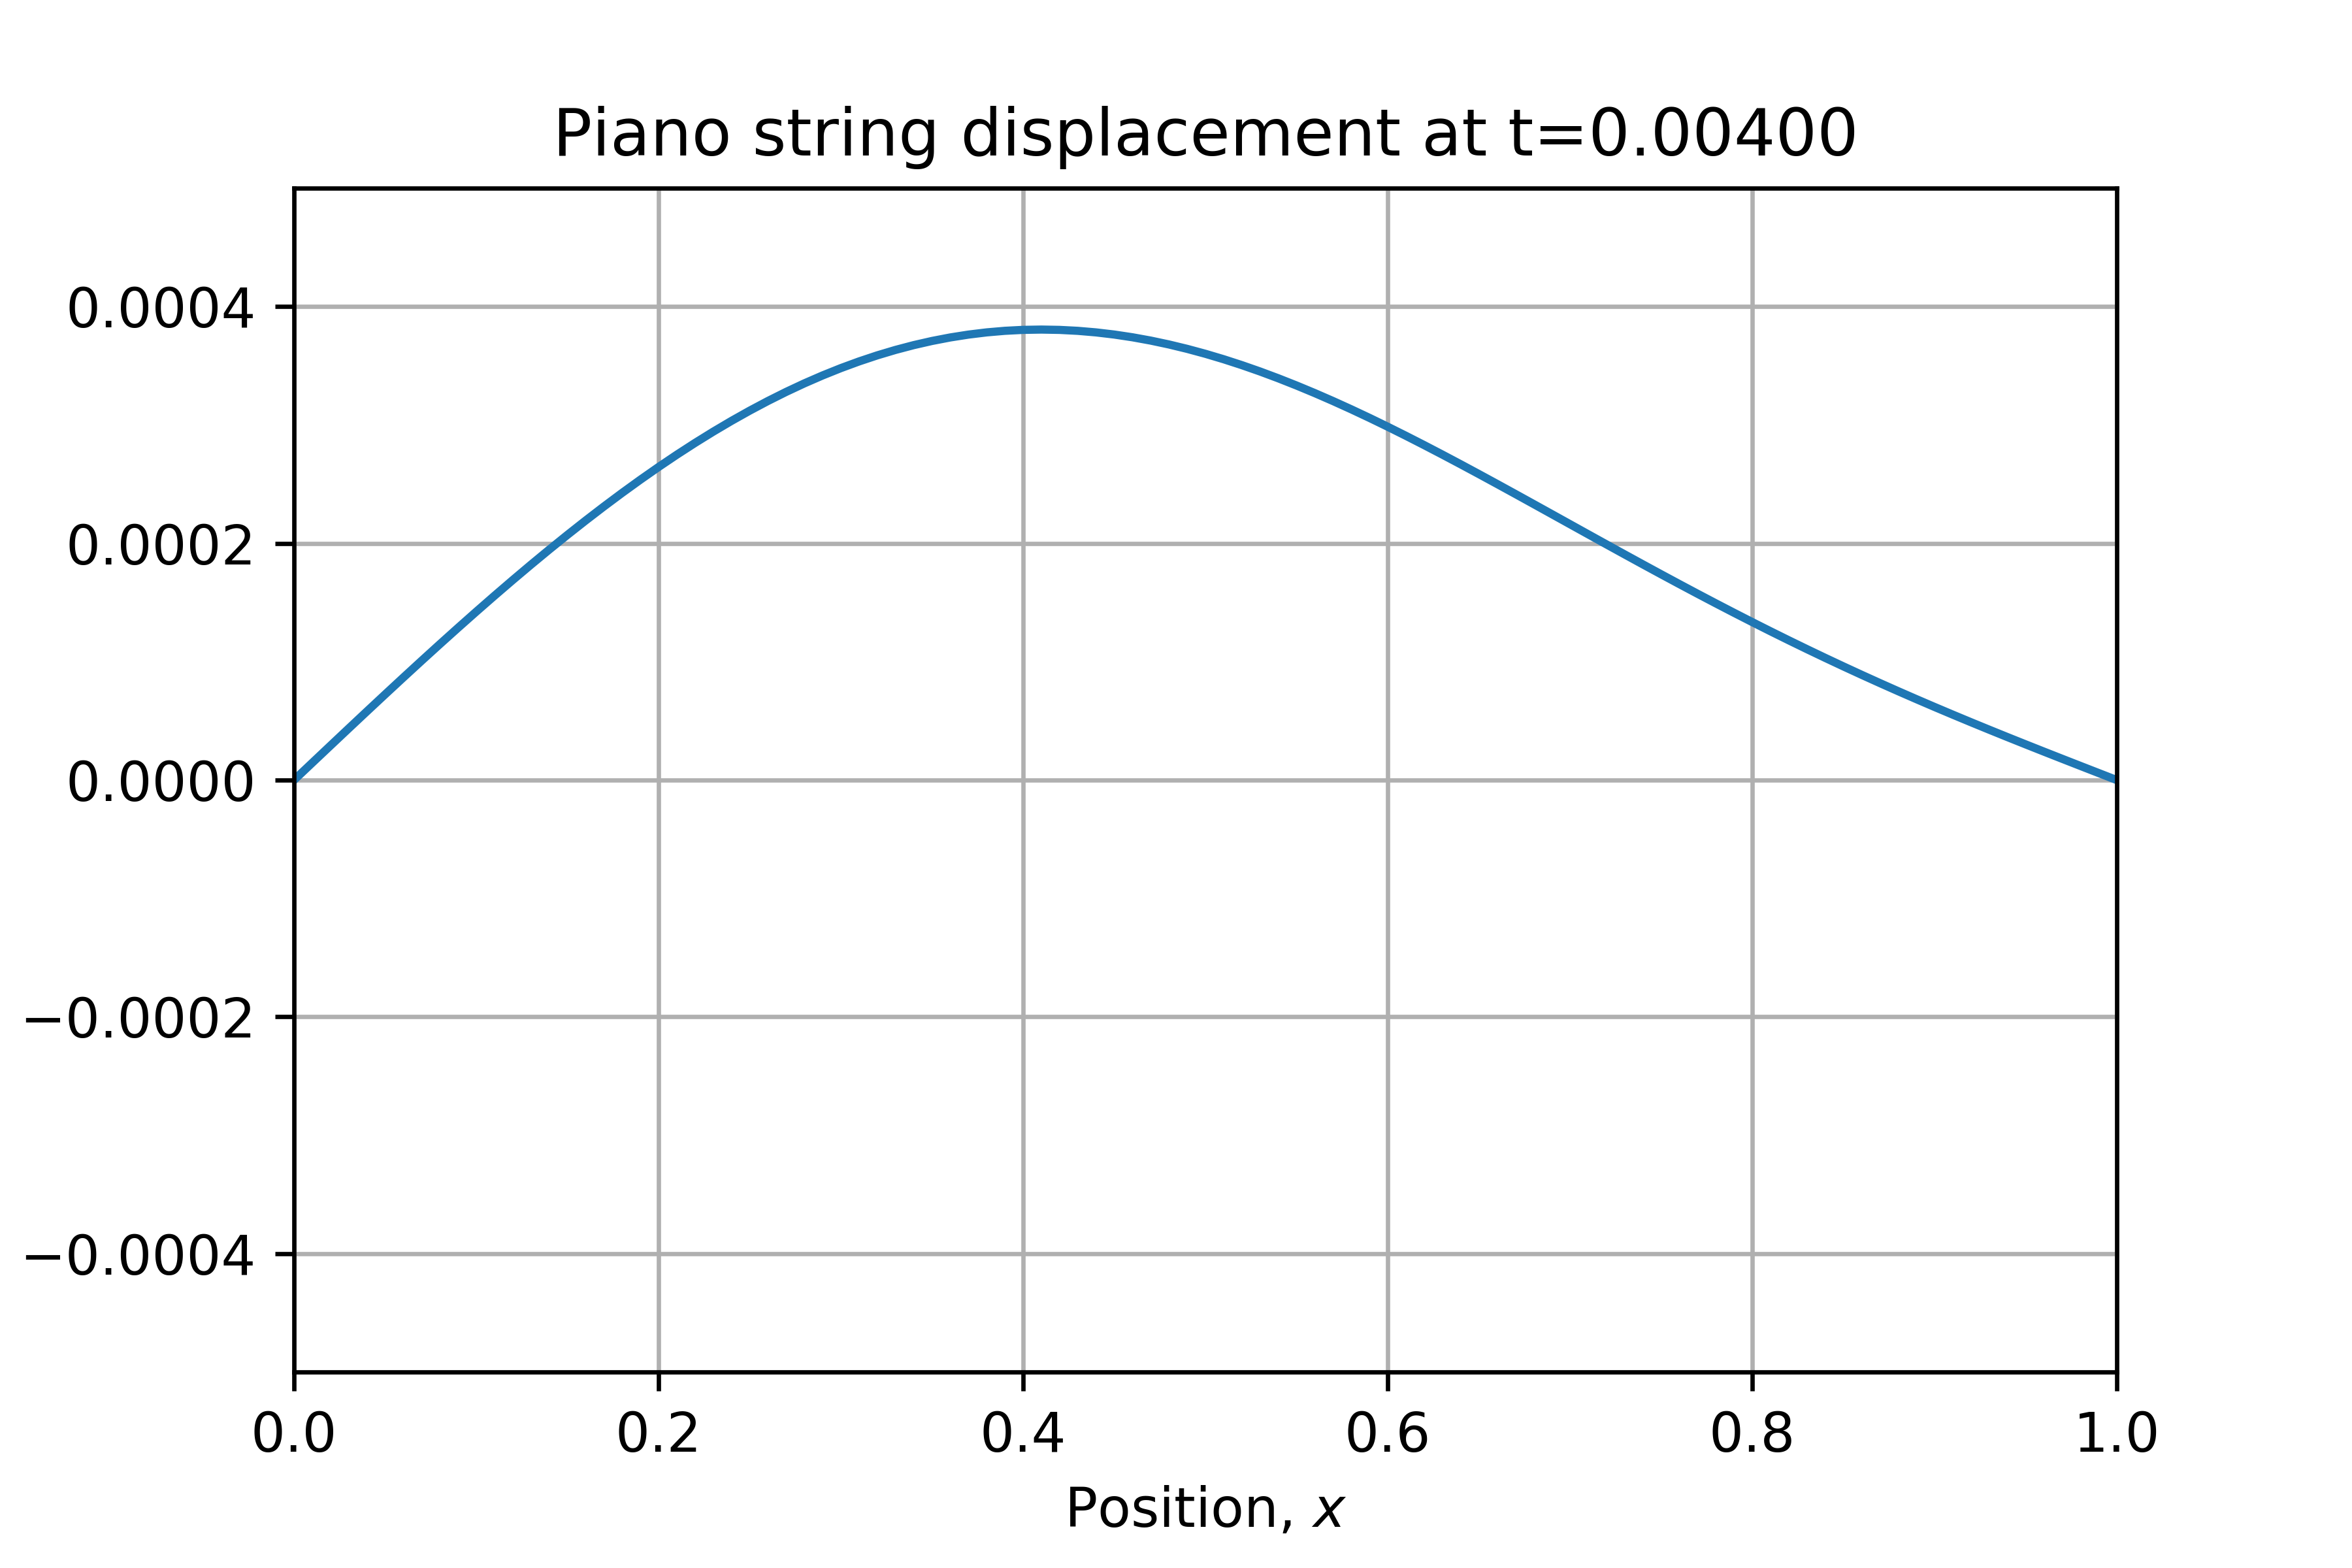
\includegraphics[width=1.0\linewidth]{../images/Lab08_t=4ms.png} 
  	\end{minipage} 
  	\begin{minipage}[b]{0.33\linewidth}
    	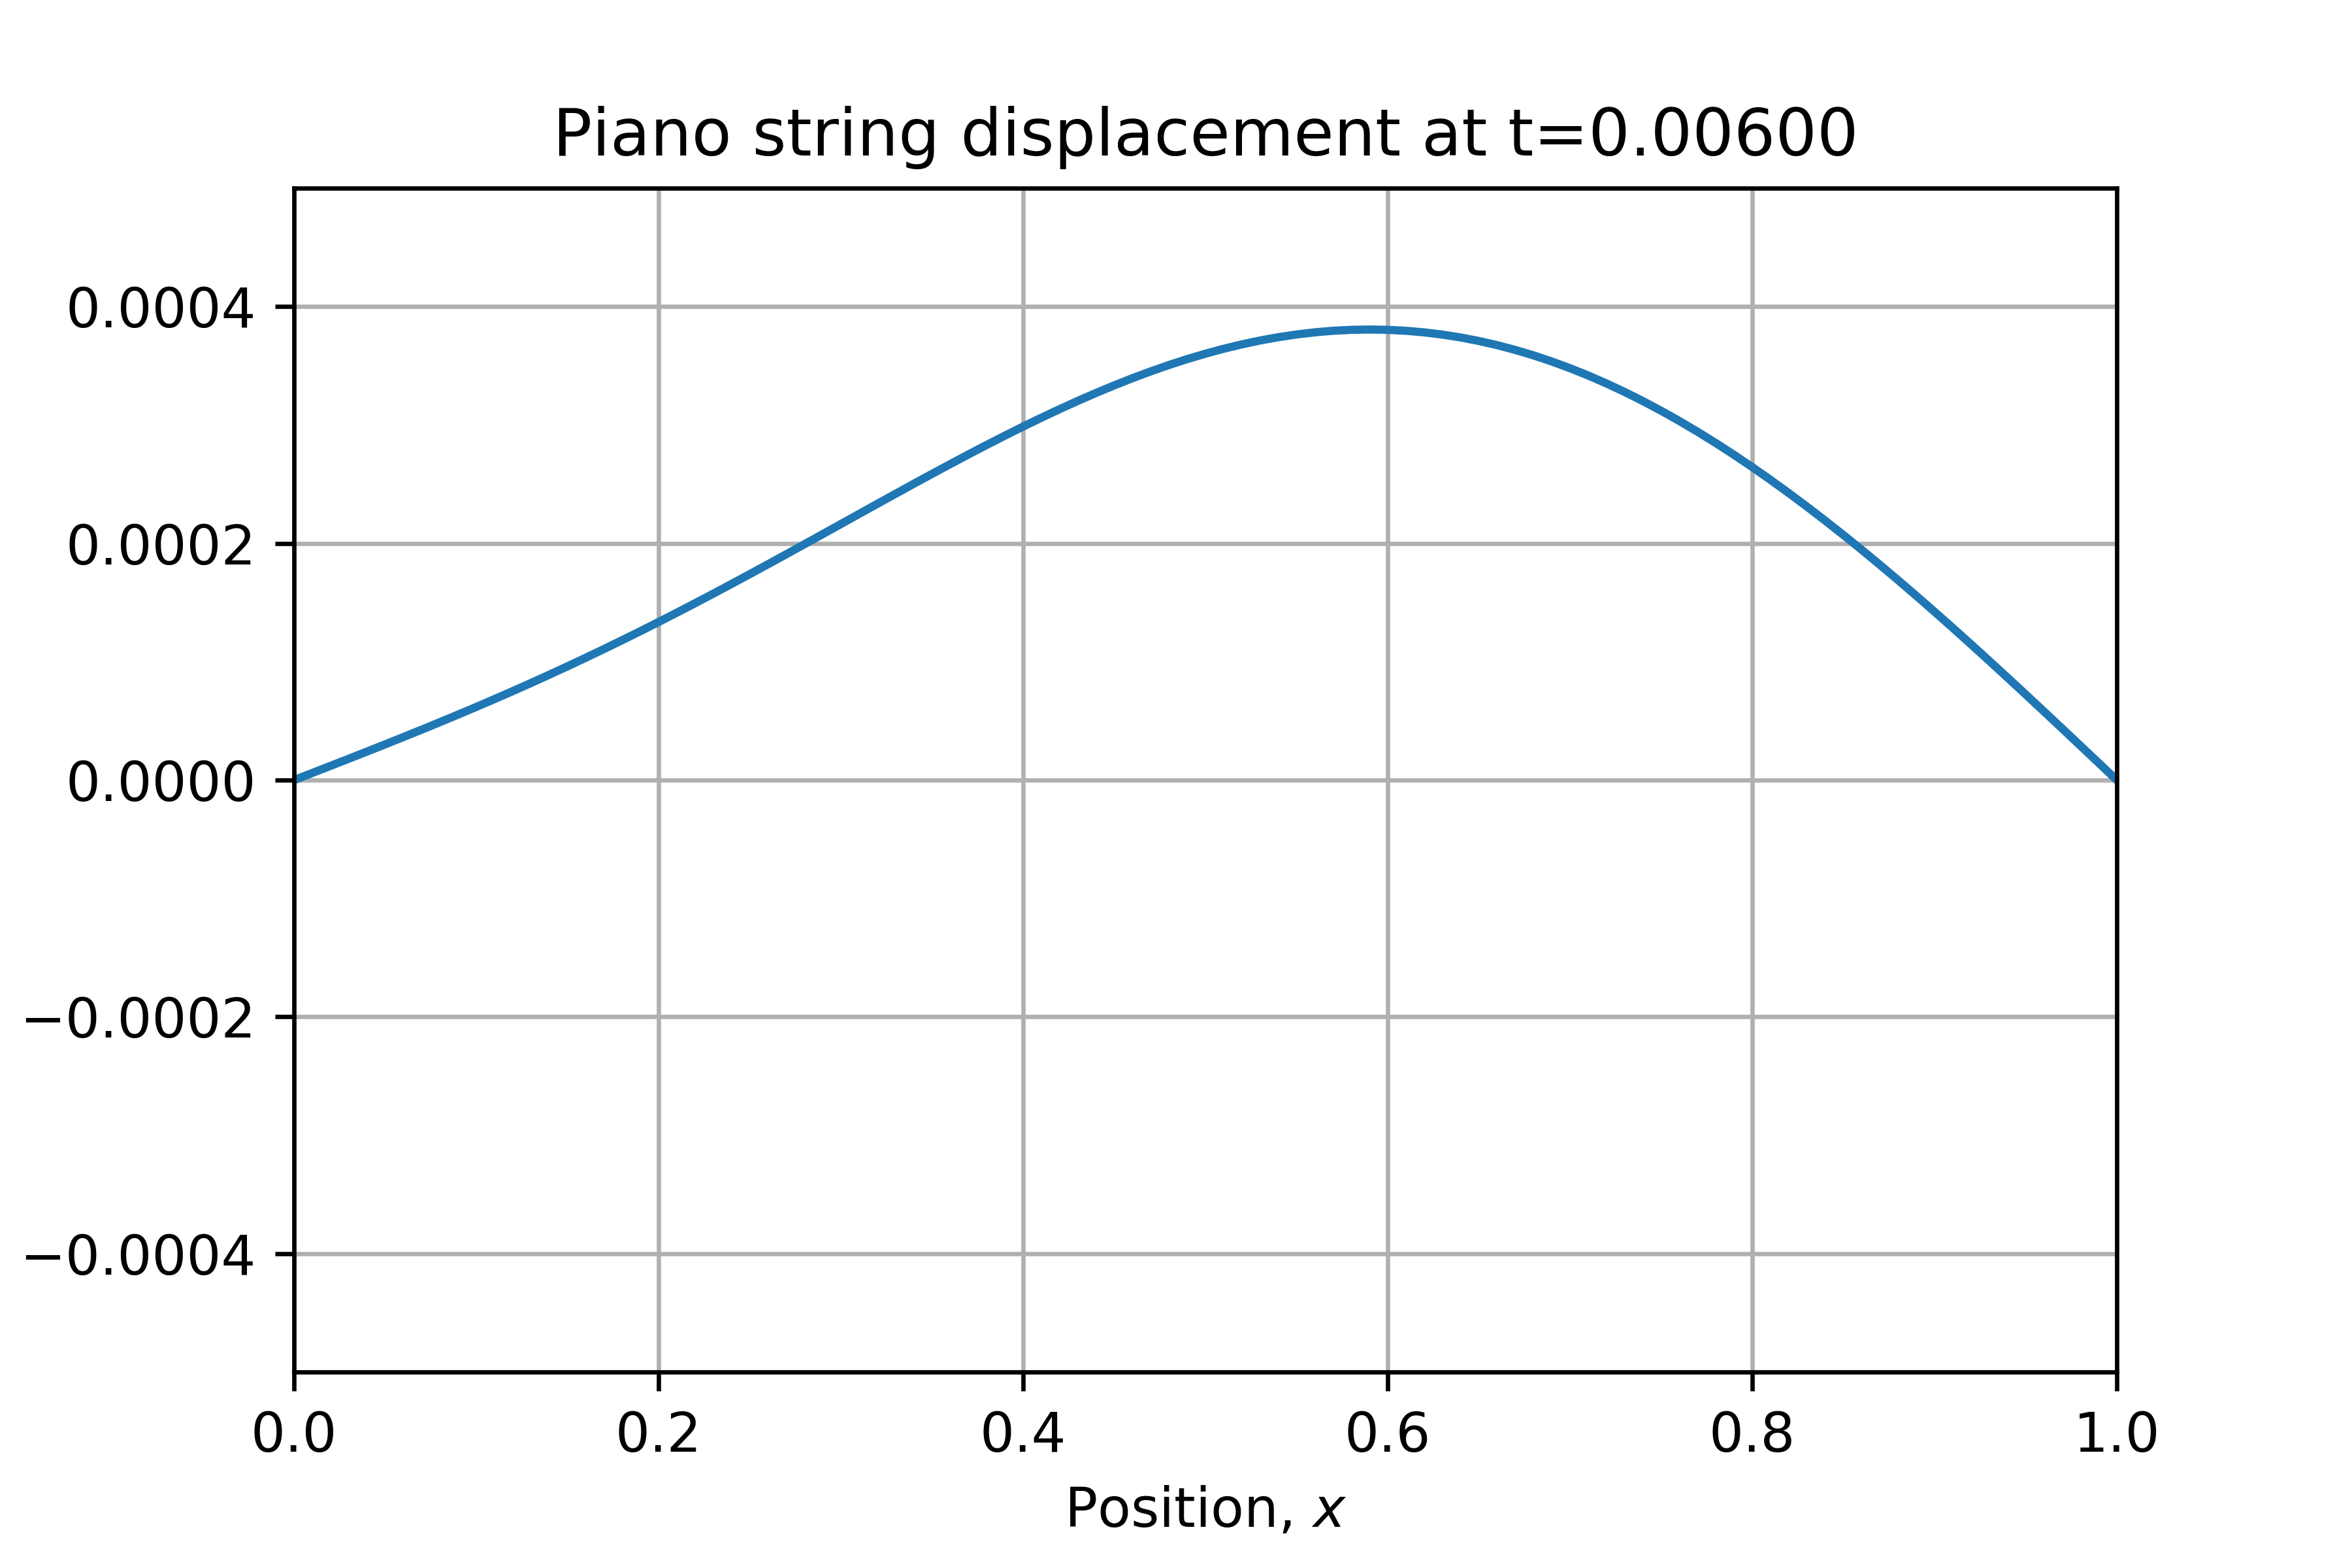
\includegraphics[width=1.0\linewidth]{../images/Lab08_t=6ms.png}
  	\end{minipage}
  	\begin{minipage}[b]{0.33\linewidth}
    	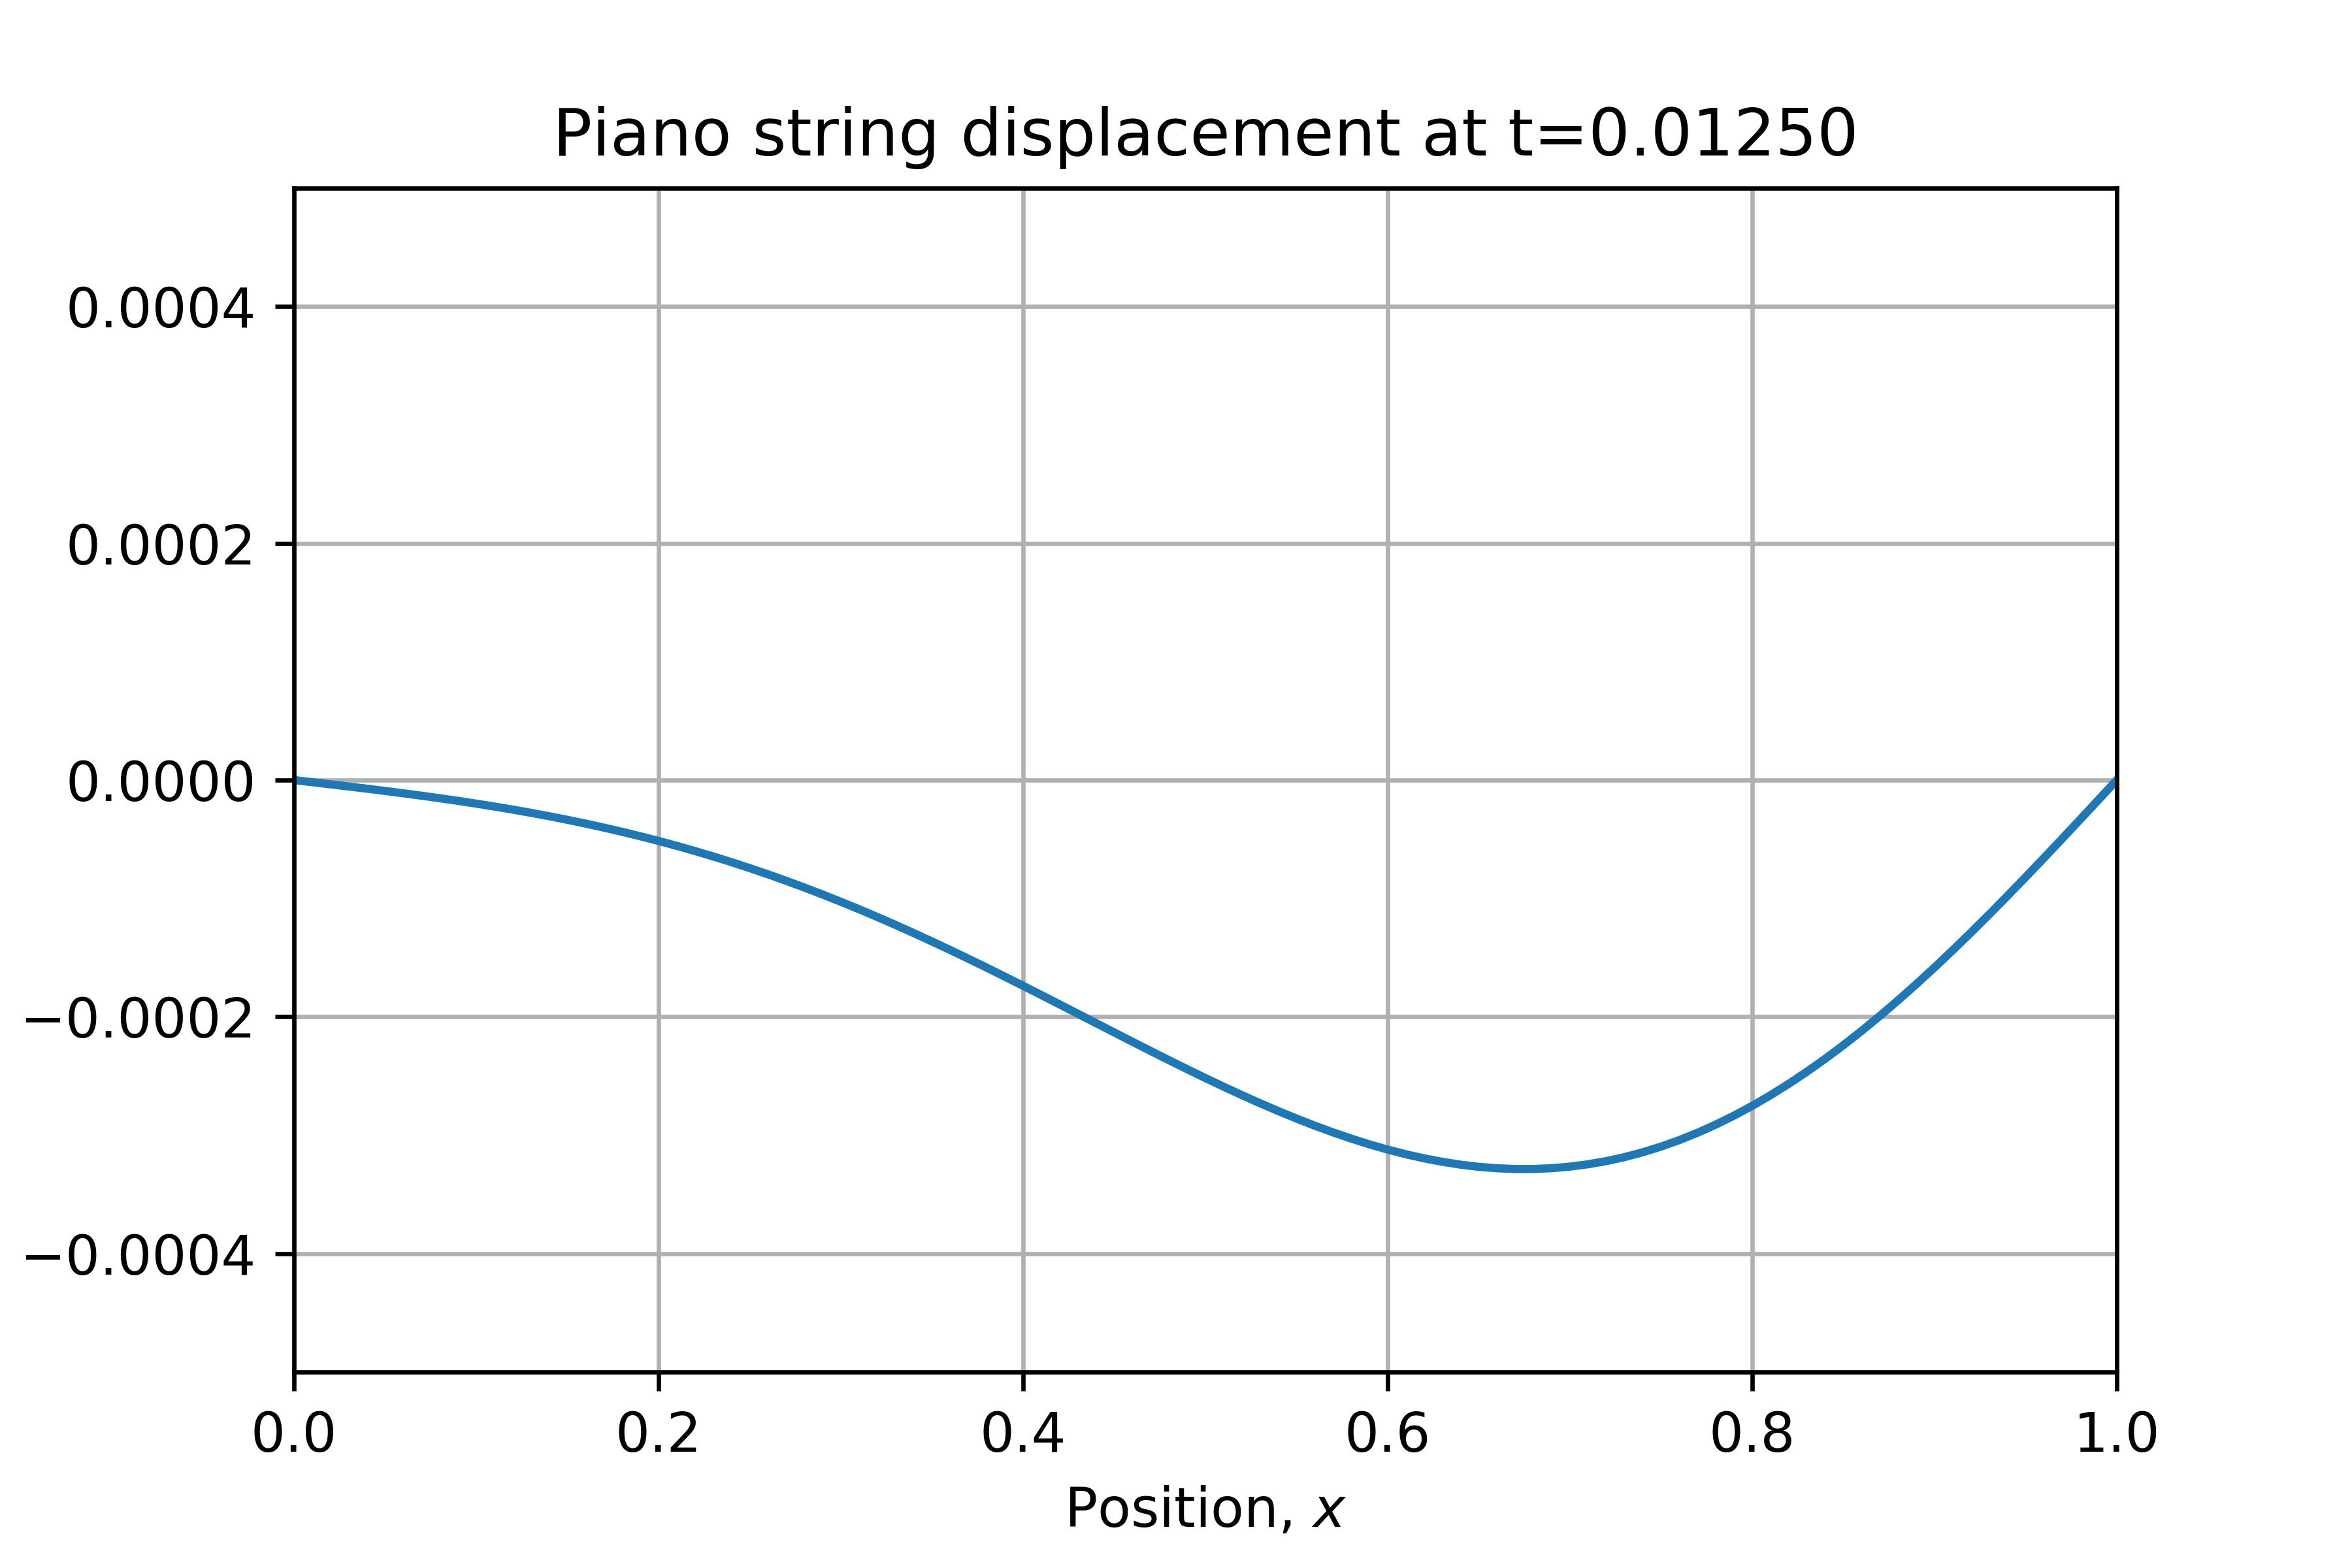
\includegraphics[width=1.0\linewidth]{../images/Lab08_t=12ms.png} 
  	\end{minipage}
  	\begin{minipage}[b]{0.33\linewidth}
  		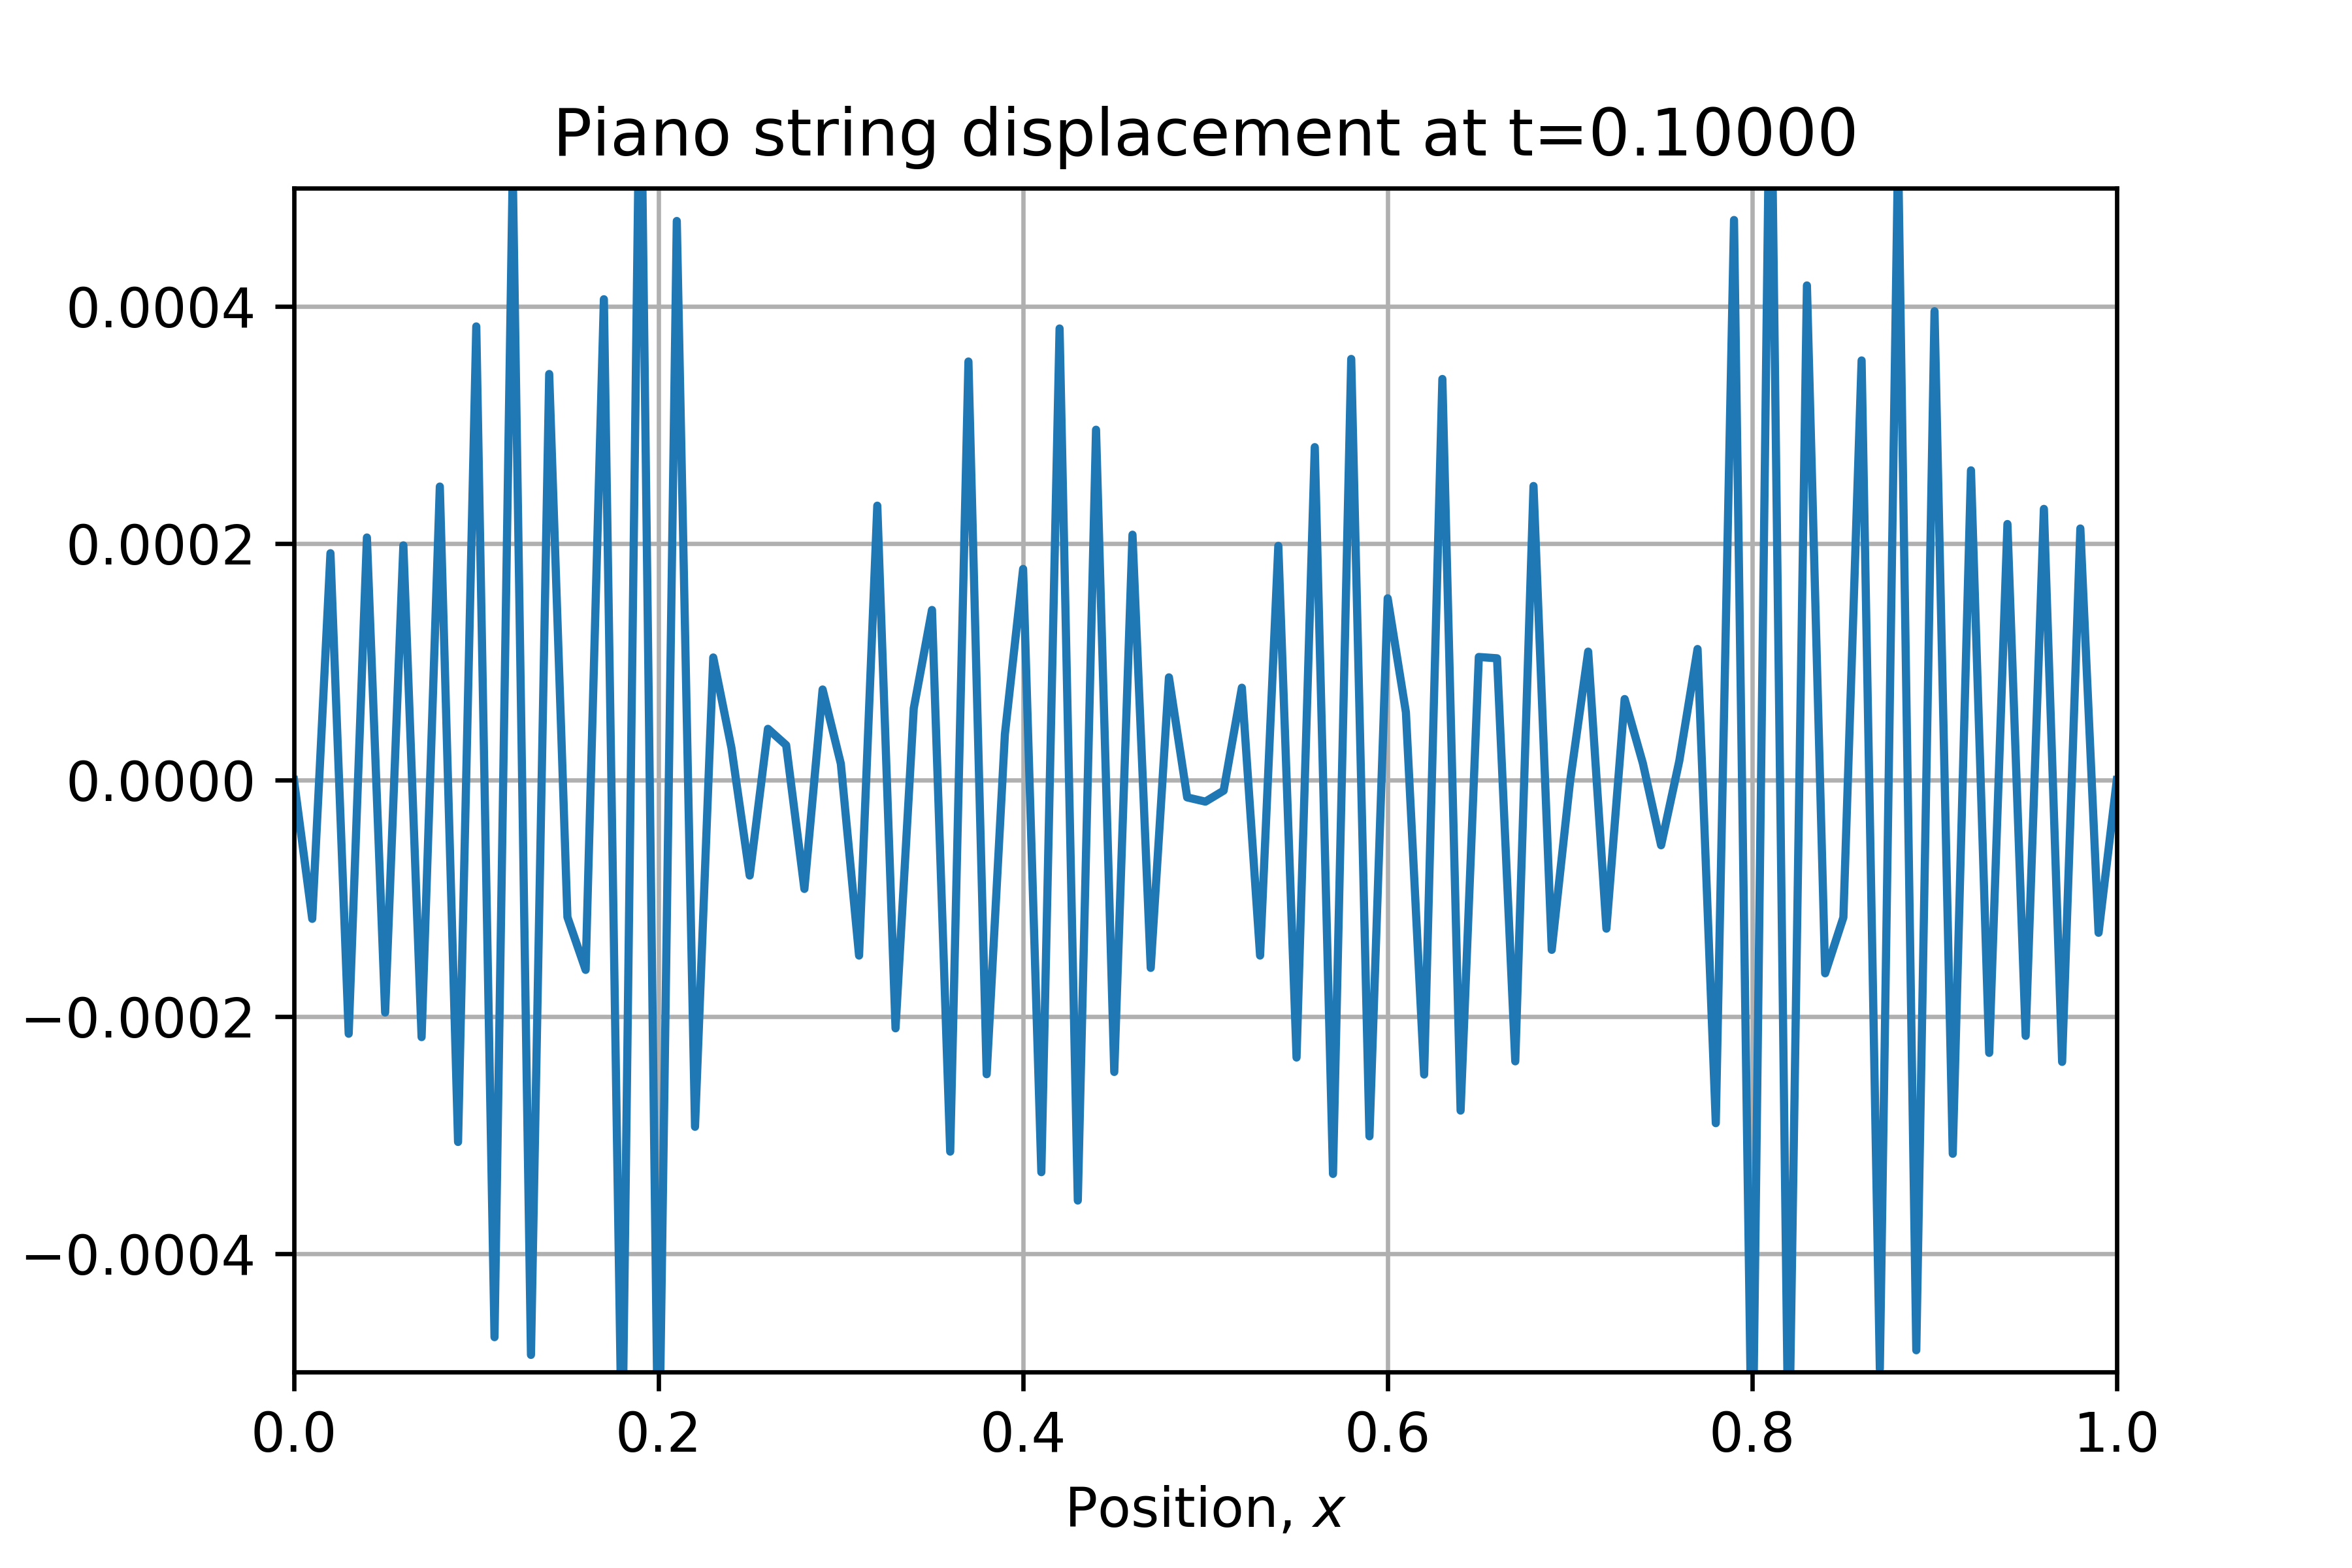
\includegraphics[width=1.0\linewidth]{../images/Lab08_t=100ms.png}
  	\end{minipage}	
 	\caption{Solutions of the wave equation applied to the displacement of a struck piano string solved using the FTCS method from Lab08, plotted at times t = 2, 4, 6, 12, 100 milliseconds.} 
\label{fig:wave_FTCS} 
\end{figure}

\section{Crank-Nicolson method}

We seek to use the Crank-Nicolson method to solve the full time-dependent Schrodinger equation in one dimension, and to animate the time evolution of a wavefunction given its initial conditions.

The code that was written to do this is attached, in Lab09\_Q2.py. The code requires ffmpeg to be downloaded with its path specified to pyplot in order to run, and outputs an mp4 of the animation up to $t=2\times 10^{-15}$s. By watching the animation, we see that the wavefunction moves to the right as time goes on, while also spreading out. When it hits the right wall, it is reflected back and travels to the left, interfering with itself in the process. This behaviour makes sense given what we know about quantum mechanics - the particle represented by the wavefunction would start with some approximate position and velocity in the center of the well, and then its probability density function, given by $|\psi|^2$, both moves to the right (the direction of its velocity) and gets broader over time.

Screenshots of the wavefunction are provided at times $t=0$s, $t=1\times 10^{-16}$s, and $t=1\times 10^{-15}$s in figures \ref{fig:q2_t=0}, \ref{fig:q2_t=1e-16}, and \ref{fig:q2_t=1e-15} respectively. From these we can see the general behaviour of the wavefunction as a function of time, and that it moves to the right until bouncing off the wall, and also spreads out as time goes on.

\begin{figure}[H]
	\centering
	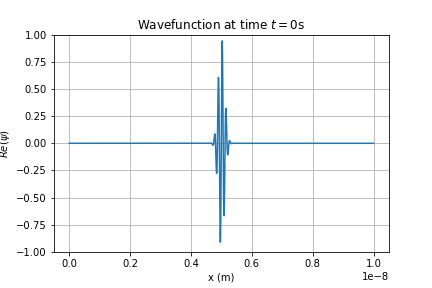
\includegraphics[width=0.8\textwidth]{../images/q2_t=0.png}
	\caption{Snapshot of wavefunction at $t=0$s.}
	\label{fig:q2_t=0}
\end{figure}

\begin{figure}[H]
	\centering
	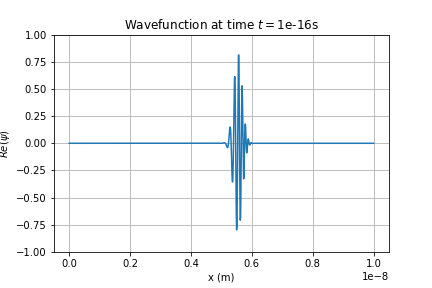
\includegraphics[width=0.8\textwidth]{../images/q2_t=1e-16.png}
	\caption{Snapshot of wavefunction at $t=1\times 10^{-16}$s.}
	\label{fig:q2_t=1e-16}
\end{figure}

\begin{figure}[H]
	\centering
	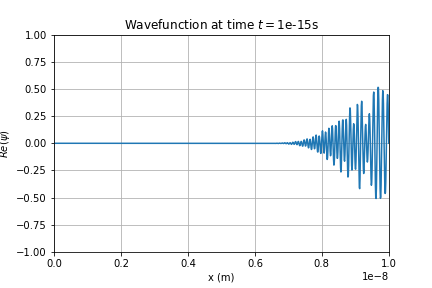
\includegraphics[width=0.8\textwidth]{../images/q2_t=1e-15.png}
	\caption{Snapshot of wavefunction at $t=1\times 10^{-15}$s.}
	\label{fig:q2_t=1e-15}
\end{figure}

\section{Solving Burger's equation using Lax-Wendroff}
For this question we desire to solve again solve Burger's equation but using the Lax-Wendroff method, to be derived, in place of the leapfrog method used in Lab08.

\subsection{Part a)}
We now concisely derive the Lax-Wendroff method as described in the lab manual. We begin with the general Taylor expansion given as 

\begin{equation}
	f(z) = f(a) + \frac{f'(a)}{1!}(z-a) + \frac{f''(a)}{2!}(z-a)^2
\end{equation}

where $f'(z)$ is the derivative with respect to time, and convert this to the desired form by replacing $z$ with $t+\Delta t$, replacing $a$ with $t$, and replacing $f(t+\Delta t)$ with $u(x, t+\Delta t)$ to get

\begin{equation}
	\label{eq:t-exp}
	u(x,t+\Delta t) = u(x,t) + u'(x,t)\Delta t + \frac{u''(x,t)}{2}\Delta t^2
	= u(x,t) + \frac{\partial u}{\partial t}\Delta t + \frac{\partial u}{\partial t}\frac{\Delta t^2}{2}
\end{equation}

Next we take Burger's equation

\begin{equation}
	\frac{\partial u}{\partial t}+\epsilon \frac{\partial u}{\partial x} \left(\frac{u^2}{2}\right) = 0
\end{equation}

and take the derivative with respect to $t$  and substitute Burger's equation back in to get

\begin{equation}
\begin{split}
	\label{eq:2nd_ord_t}
	\frac{\partial^2 u }{\partial t^2} =& - \epsilon \frac{\partial }{\partial t}\frac{\partial }{\partial x} \left(\frac{u^2}{2} \right)
	= - \epsilon \frac{\partial }{\partial x}\frac{\partial }{\partial t} \left(\frac{u^2}{2} \right)
	= - \frac{\epsilon}{2} \frac{\partial }{\partial x}\left( 2u\frac{\partial u}{\partial t} \right)
	\\ =& - \epsilon \frac{\partial }{\partial x} \left( u \left[ -\epsilon \frac{\partial }{\partial x} \left(\frac{u^2}{2} \right) \right] \right)
	= \epsilon^2 \frac{\partial}{\partial x} \left[u \frac{\partial}{\partial x}\left( \frac{u^2}{2}\right) \right]
\end{split}
\end{equation}

We then substitute Burger's equation for the first order time derivative in equation \ref{eq:t-exp} and substitute equation \ref{eq:2nd_ord_t} for the second order time derivative to get

\begin{equation}
	\label{eq:t_exp_2}
	u(x,t+\Delta t) = u(x,t) - \epsilon \Delta t \frac{\partial }{\partial x} \left(\frac{u^2}{2}\right) + \frac{(\epsilon\Delta t)^2}{2}\frac{\partial}{\partial x }\left(u\frac{\partial}{\partial x}\left(\frac{u^2}{2}\right) \right)
\end{equation}

We then use the central difference approximation defined as 

\begin{equation}
	f(x) = \frac{f(x+h/2) - f(x-h/2)}{h}
\end{equation}

and replace $h$ with $2\Delta x$ and $f(x)$ with $u^2(x,t)$ to get 

\begin{equation}
	\frac{\partial u^2(x,t)}{\partial x} = \frac{u^2(x+\Delta x, t) - u^2(x-\Delta x, t)}{2\Delta x}
\end{equation}

Equation \ref{eq:t_exp_2} then becomes

\begin{equation}
\begin{split}
	\label{eq:t_exp_3}
	u(x,t+\Delta t) = u(x,t) - \frac{\epsilon \Delta t}{2} \left[ \frac{u^2(x+\Delta x, t) - u^2(x-\Delta x, t)}{2\Delta x} \right] + \frac{(\epsilon\Delta t)^2}{4}\frac{\partial}{\partial x }\left[u\frac{\partial}{\partial x}\left(\frac{u^2}{2}\right) \right]
\end{split}
\end{equation}

Applying the central difference approximation again but this time using $h=\Delta x/2$ and $f(x)=u(x,t)\frac{\partial u^2(x,t)}{\partial x}$ we get 

\begin{equation}
	\frac{\partial}{\partial x}\left(u\frac{\partial u^2}{\partial x} \right) = \frac{1}{\Delta x} \left[u(x+\Delta x/2)\frac{\partial u^2(x+\Delta x/2, t)}{\partial x} - u(x-\Delta x/2, t)\frac{\partial u^2(x-\Delta x/2, t)}{\partial x} \right]
\end{equation}

which we substitute into equation \ref{eq:t_exp_3} to get

\begin{equation}
\begin{split}
	u(x,t+\Delta t) = & u(x,t) - \frac{\epsilon \Delta t}{4 \Delta x} \left[ u^2(x+\Delta x, t) - u^2(x-\Delta x, t) \right] 
	\\ & + \frac{(\epsilon\Delta t)^2}{4}\frac{1}{\Delta x} \left[u(x+\Delta x/2)\frac{\partial u^2(x+\Delta x/2, t)}{\partial x} - u(x-\Delta x/2, t)\frac{\partial u^2(x-\Delta x/2, t)}{\partial x} \right]
\end{split}
\end{equation}

Using the average centered on $u(x\pm \Delta x/2)$ we have
\begin{equation}
	u(x\pm \Delta x/2, t) = \frac{u(x,t)+u(x\pm \Delta x,t)}{2}
\end{equation}

giving us

\begin{equation}
\begin{split}
	u(x,t+ \Delta t) = & u(x,t) - \frac{\epsilon \Delta t}{4 \Delta x} \left[ u^2(x+ \Delta x, t) - u^2(x- \Delta x, t) \right] 
	\\ & + \frac{(\epsilon \Delta t)^2}{4 \Delta x} \left[ (u(x,t)+u(x+ \Delta x,t))\frac{\partial u^2(x+ \Delta x/2, t)}{\partial x} - (u(x,t)+u(x- \Delta x,t)) \frac{\partial u^2(x- \Delta x/2, t)}{\partial x} \right]
\end{split}
\end{equation}

Using the central difference approximation a third time for $h=\pm \Delta x$ and $f(x)=u^2(x\pm \Delta x/2, t)$ we have

\begin{equation}
	\frac{\partial u^2(x \pm \Delta x/2, t)}{\partial x} = \frac{u^2(x \pm \Delta x, t) - u^2(x,t)}{\pm \Delta x}
\end{equation}

and our Lax-Wendroff method becomes

\begin{equation}
\begin{split}
	u(x,t+ \Delta t) = & u(x,t) -  \frac{\epsilon \Delta t}{4 \Delta x} \left[ u^2(x+ \Delta x, t) - u^2(x- \Delta x, t) \right] 
	\\ & + \frac{(\epsilon \Delta t)^2}{8 \Delta x^2} \Big([u(x,t)+u(x+ \Delta x,t)] [u^2(x + \Delta x, t) - u^2(x,t)] 
	\\ & + [u(x,t)+ u(x-\Delta x,t)][ u^2(x - \Delta x, t) - u^2(x,t) ]\Big)
\end{split}
\end{equation}

which we can simplify using the notation
\begin{equation}
	u(x,t) = u^j_i
\end{equation}
where $i+n = x+n \Delta x$ and $j+m = x+m \Delta t$.

Our final equation is then

\begin{equation}
	u^{j+1}_i = u^j_i - \frac{\beta}{4} \left[(u^j_{i+1})^2 - (u^j_{i-1})^2 \right] + \frac{\beta^2}{8} \left[ (u^j_i+u^j_{i+1}) ((u^j_{i+1})^2 - (u^j_i)^2) + (u^j_i + u^j_{i-1})((u^j_{i-1})^2 - (u^j_i)^2) \right]
\end{equation}

where $\beta = \epsilon \Delta t/\Delta x$. This is the form of the Lax-Wendroff method that will be used in place of the leapfrog method used in Lab08.

\subsection{Part b)}

Using the same basic program as used in Lab08 we have the values 

\begin{align}
	\epsilon =& 1.0 & \Delta x =& 0.02 & \Delta t =& 0.005 \\
	L_x =& 2\pi & T_f =& 2.0 & 
\end{align}

and initial condition $u(x,t=0)=sin(x)$ and boundary condition $u(x=0,t)=0=u(x=L_x,t)$. The Lax-Wendroff method is then implemented to solve the Burger's equation for the given time interval and the solutions at times $t=0, 0.5, 1.0, 1.5$ are plotted and shown in figure \ref{fig:burgers_lax}. Comparing this solution to that of Lab08 shown in figure \ref{fig:burgers_leapfrog} we can see what we suspected last week, namely, the the shock depicted is a feature of the Burger's equation while the noise shown in the $t=1.5$ solution of the leapfrog method is an error of the implementation of the leapfrog method which vanishes when we instead use the Lax-Wendroff method for our solutions.

\begin{figure}[H]
	\centering
	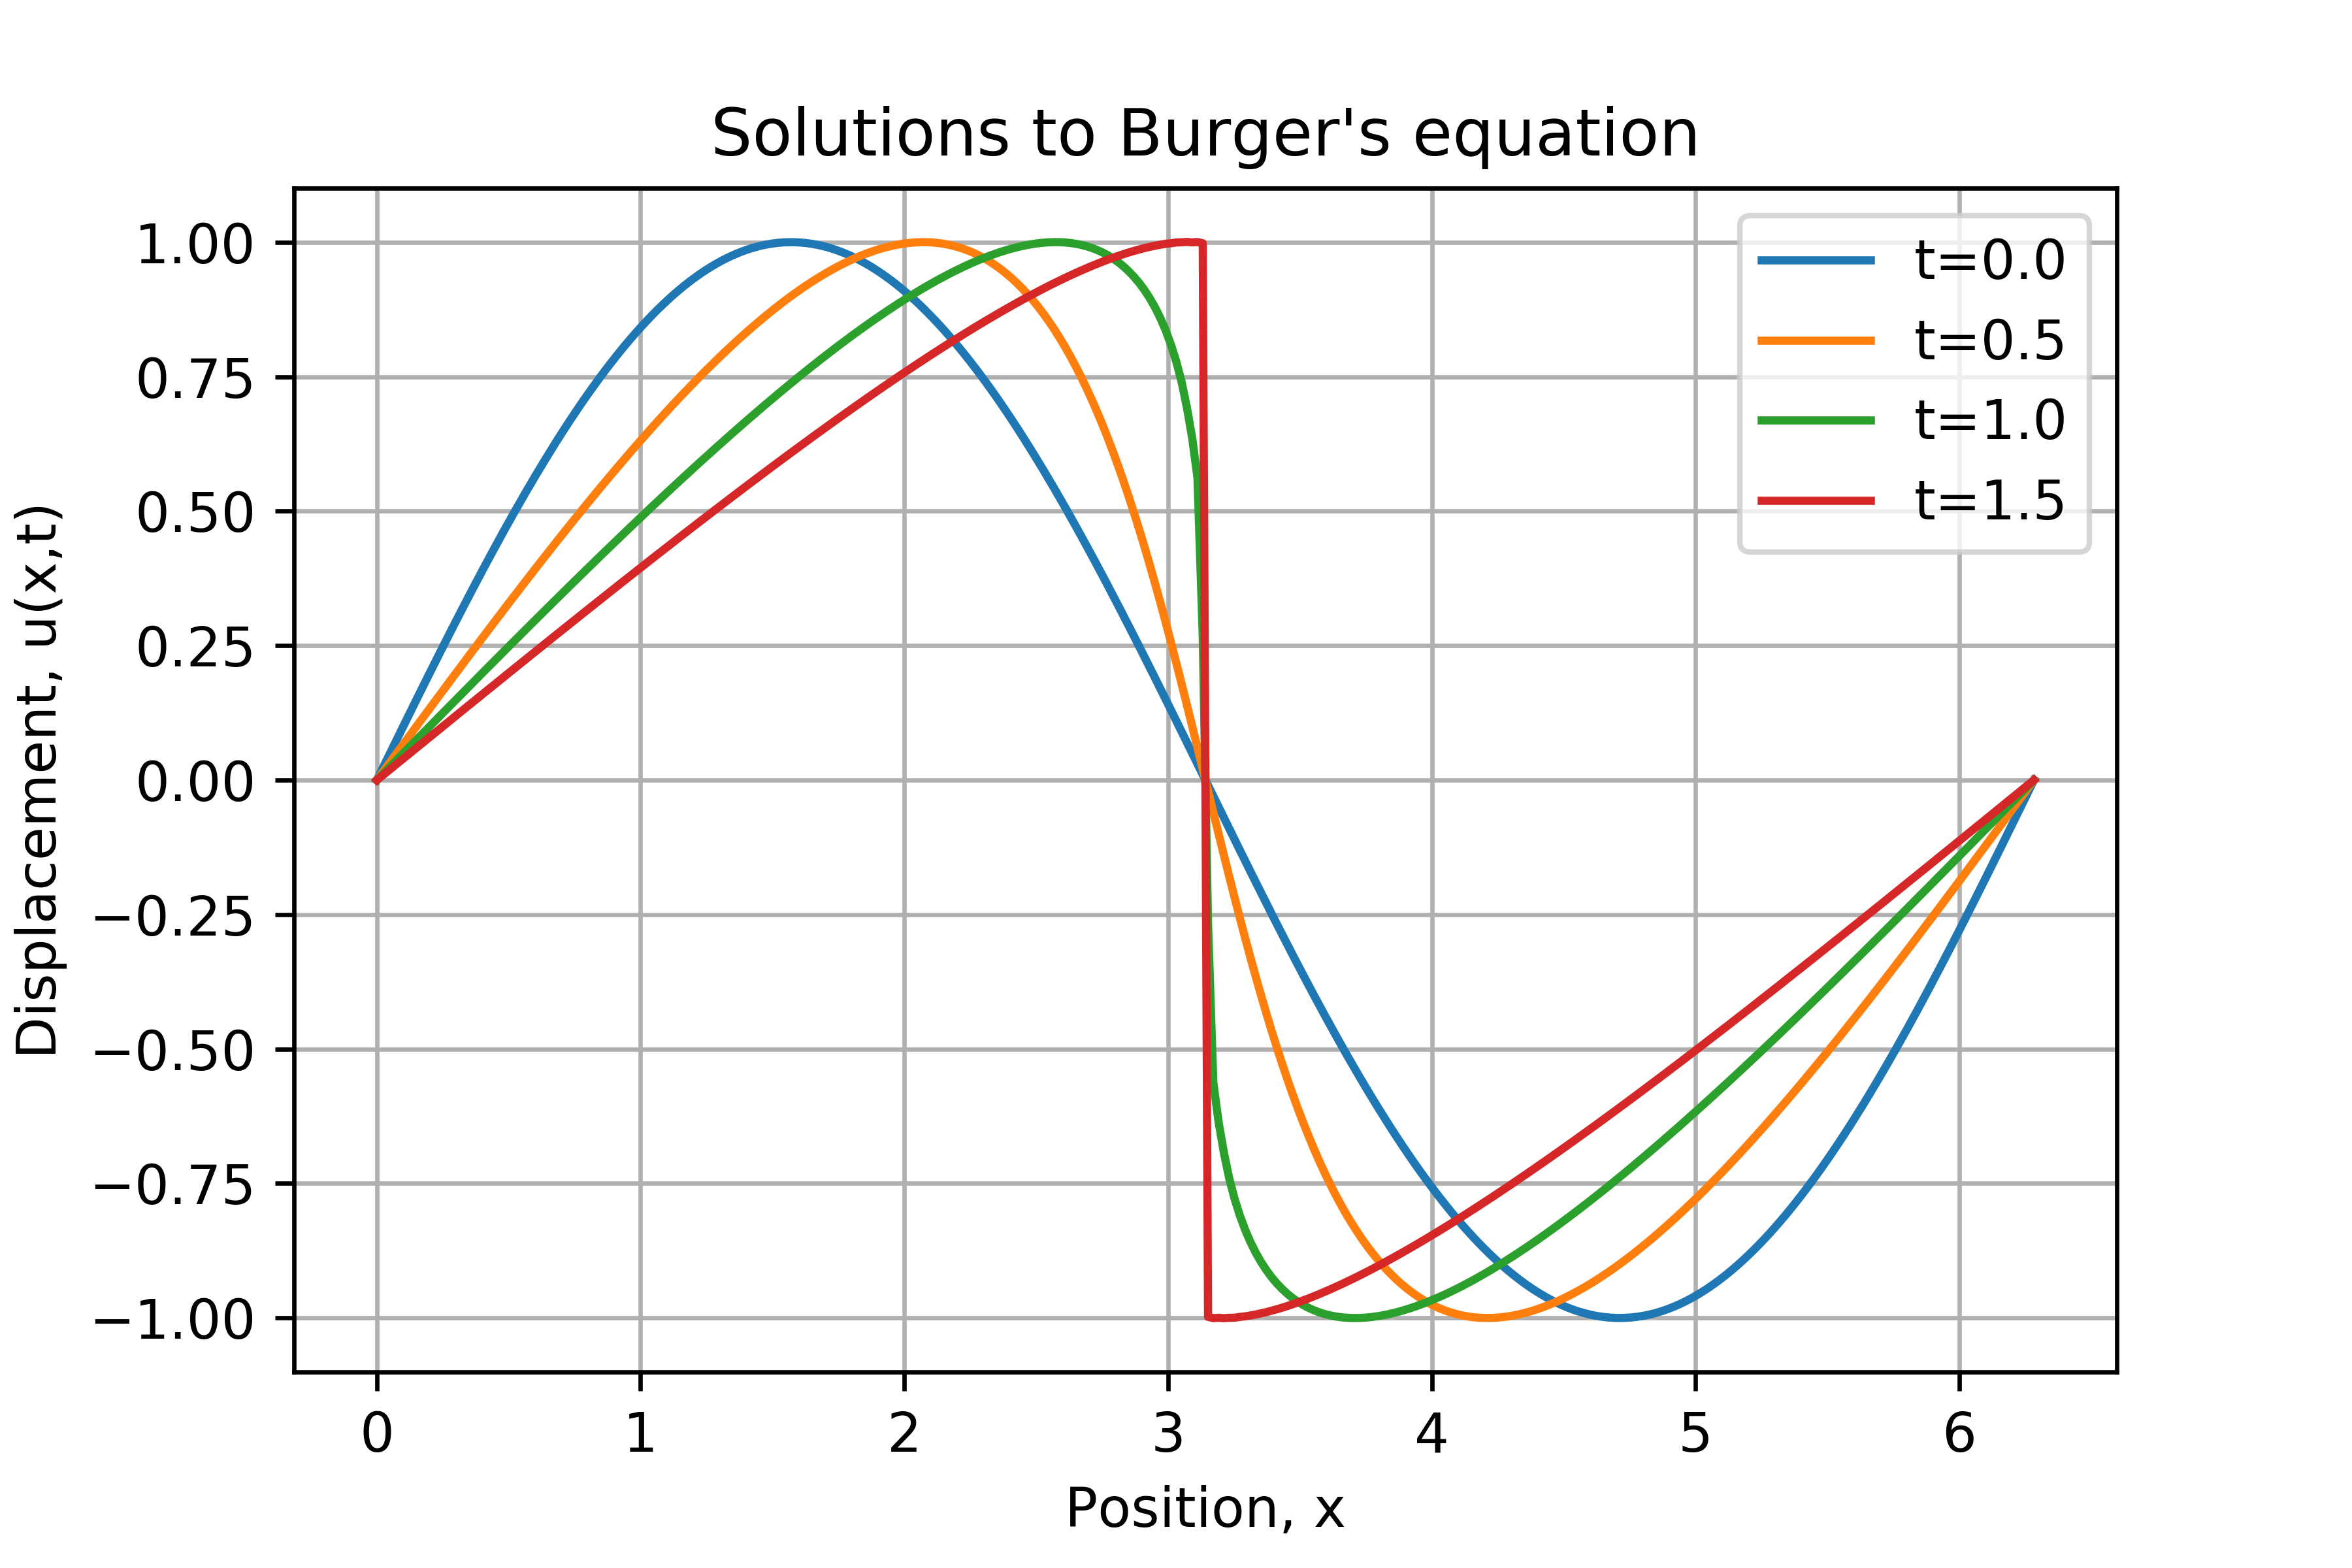
\includegraphics[width=0.8\textwidth]{../images/burgers.png}
	\caption{Plot of the solution of Burger's equation using the Lax-Wendroff method for times $t=0.0,0.5,1.0,1.5$ using an even number of points, $N_x=314$, with $\Delta x=0.02$ and $\Delta t=0.005$.}
	\label{fig:burgers_lax}
\end{figure}

\begin{figure}[H]
	\centering
	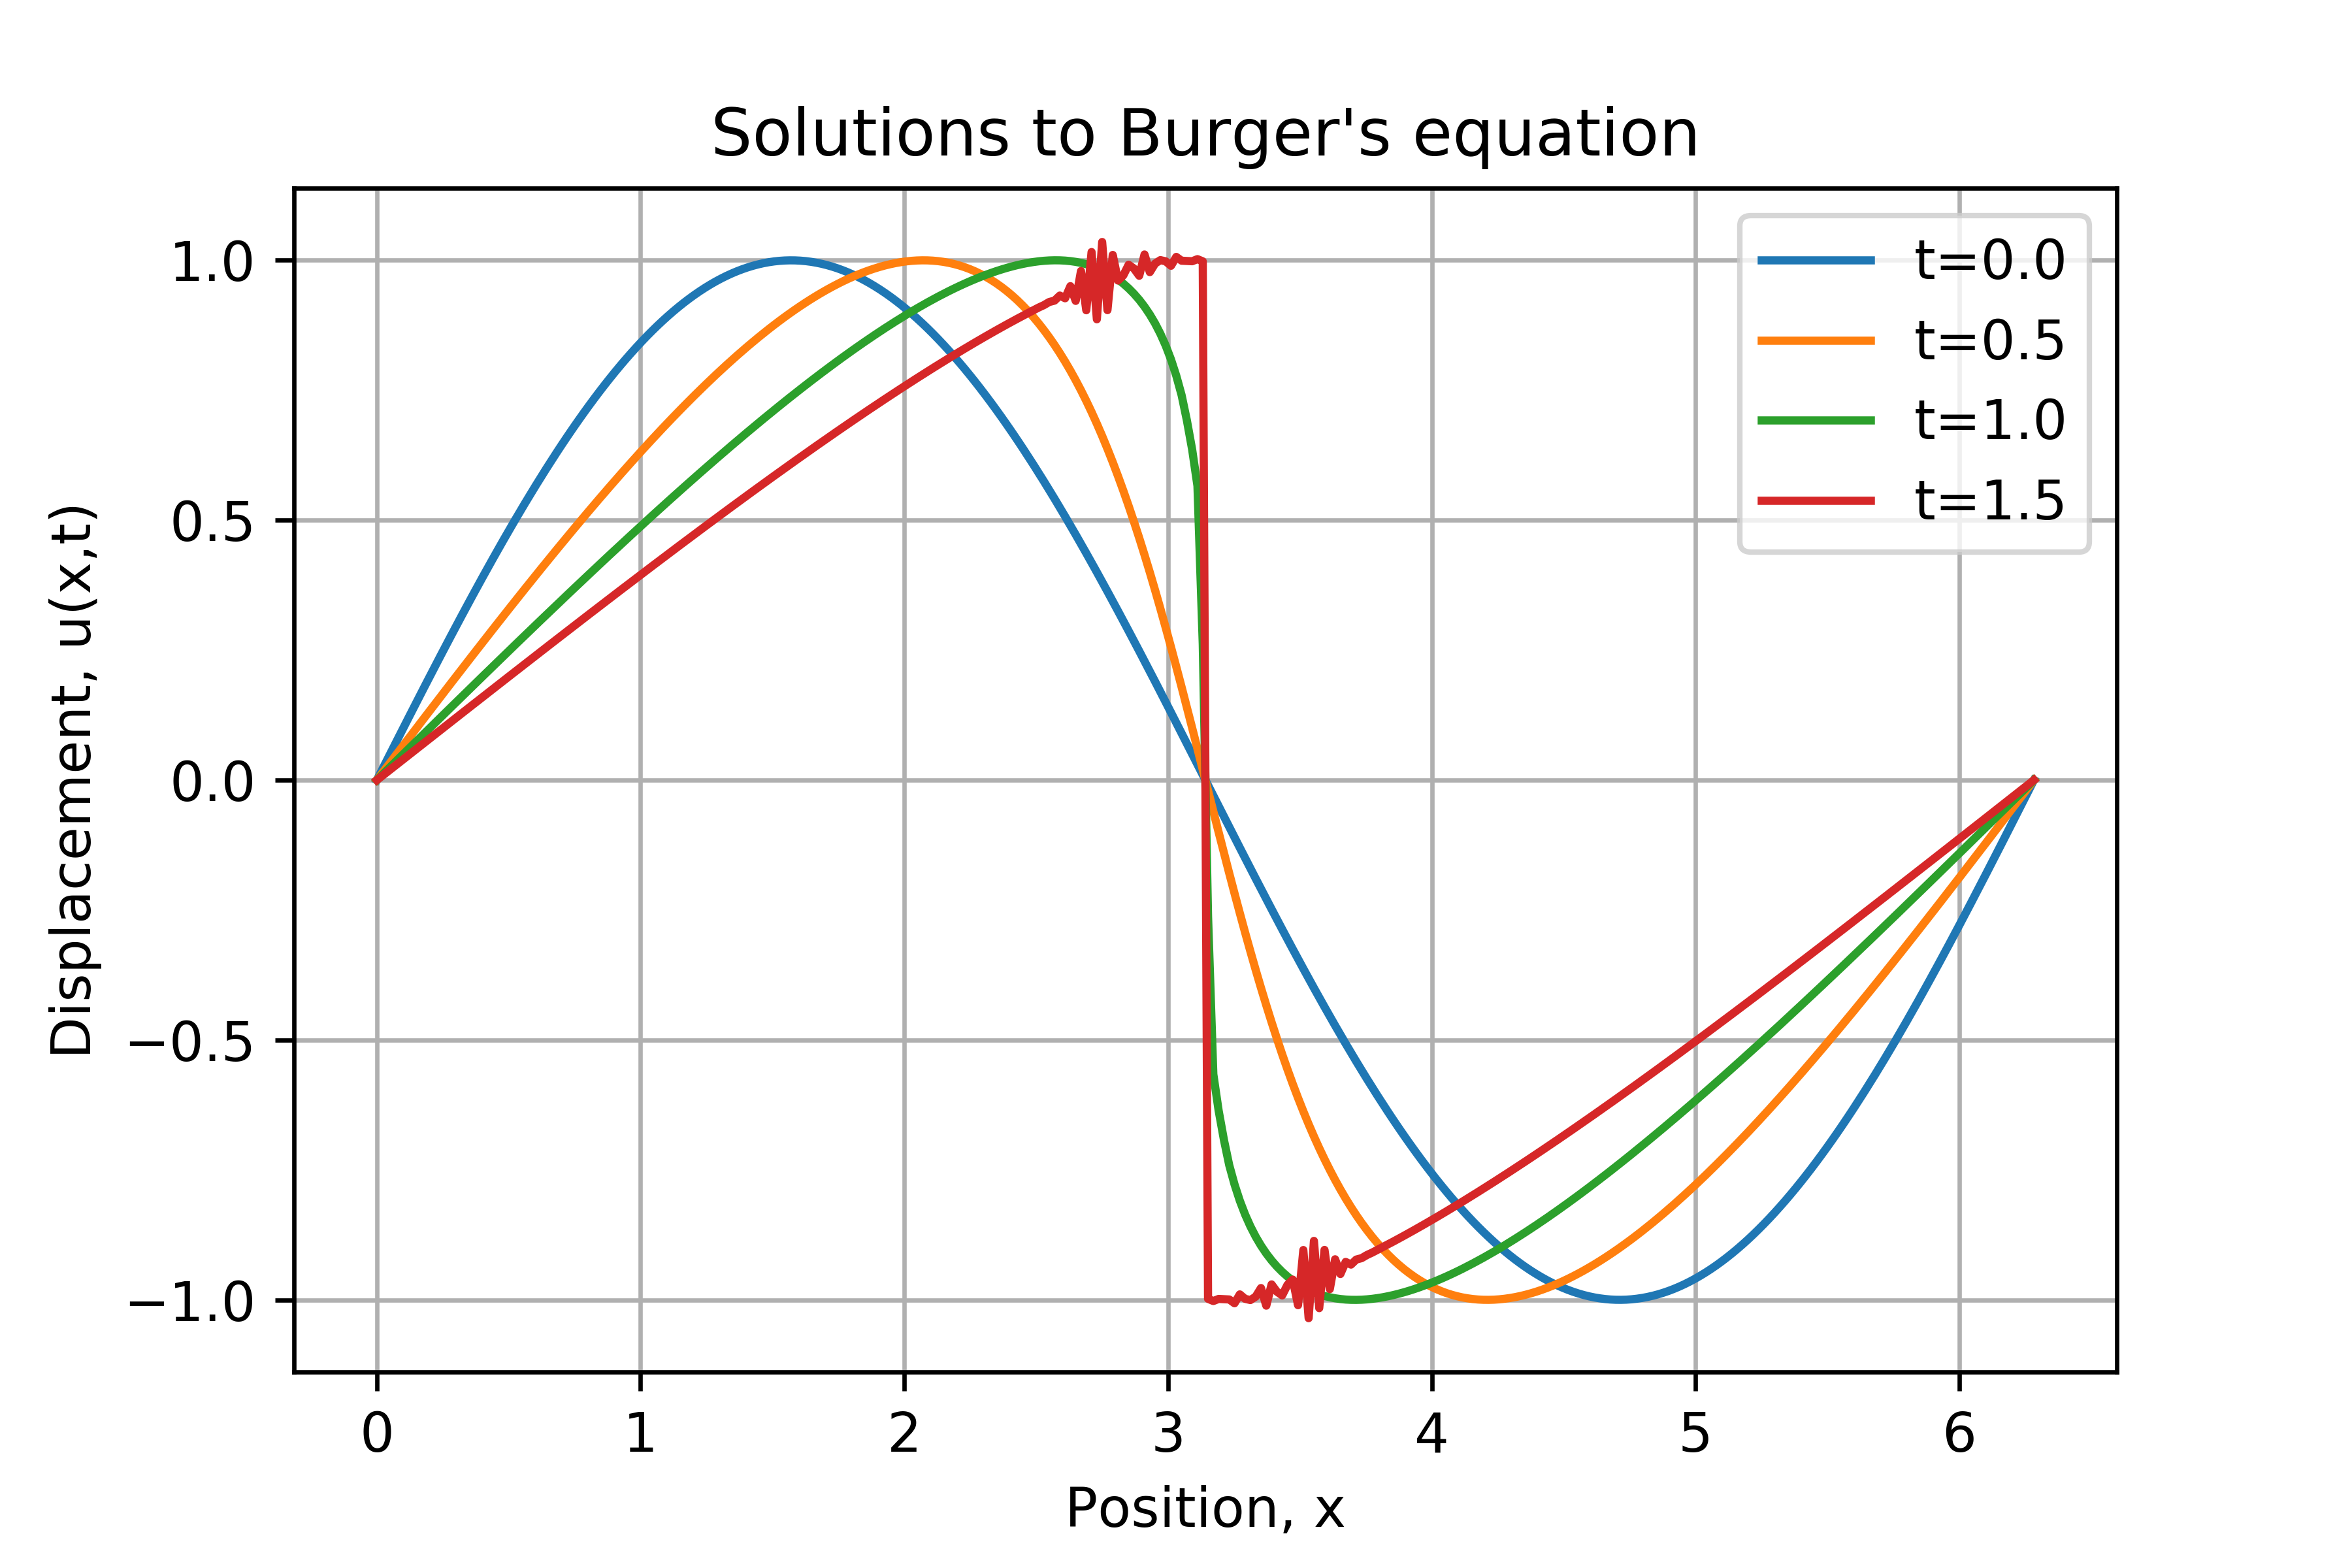
\includegraphics[width=0.8\textwidth]{../images/burgers_old.png}
	\caption{Plot of the solution of Burger's equation from Lab08 using the leapfrog method for times $t=0.0,0.5,1.0,1.5$ using an even number of points, $N_x=314$, with $\Delta x=0.02$ and $\Delta t=0.005$.}
	\label{fig:burgers_leapfrog}
\end{figure}

\end{document}